\documentclass[12pt]{article}
\usepackage{latexsym,amssymb,amsmath,amsfonts,amsthm,arydshln,calc,comment,hyperref,mathrsfs,placeins,xcolor,graphicx,longtable,bm,cite,blkarray,bbm,dsfont}
\usepackage{hyperref}
\usepackage[notref,notcite]{showkeys}
\usepackage{tikz, tikz-cd}
\usepackage{booktabs, array}
%\usetikzlibrary{matrix}
\usetikzlibrary{fit, positioning, arrows}
\hypersetup{colorlinks=true}

\usepackage{longtable} % For long tables


\setlength{\textwidth}{6.4in}
\setlength{\textheight}{8.8in}
\setlength{\topmargin}{-0.6in}
\setlength{\oddsidemargin}{.0in}
\setlength{\evensidemargin}{.0in}


%%%%%%%%%%%%%%%%%%%%%% all new theorem def

\newtheorem{theorem}{Theorem}
\numberwithin{theorem}{section} % counting in section, can also be changed by {subsection}
\newtheorem{definition}{Definition}
\numberwithin{definition}{section} % counting in section, can also be changed by {subsection}
\newtheorem{assumption}{Assumption}
\numberwithin{assumption}{section} % counting in section, can also be changed by {subsection}
\newtheorem{lemma}{Lemma}
\numberwithin{lemma}{section} % counting in section, can also be changed by {subsection}
\newtheorem{remark}{Remark}
\numberwithin{remark}{section} % counting in section, can also be changed by {subsection}
\newtheorem{prop}{Proposition}
\numberwithin{prop}{section} % counting in section, can also be changed by {subsection}
\newtheorem{corollary}{Corollary}
\numberwithin{corollary}{section} % counting in section, can also be changed by {subsection}
\newtheorem{example}{Example} 
\numberwithin{example}{section} % counting in section, can also be changed by {subsection}
\newtheorem{question}{Question} 
\numberwithin{question}{section} % counting in section, can also be changed by {subsection}
\newtheorem{problem}{Problem} 
\numberwithin{problem}{section} % counting in section, can also be changed by {subsection}
\newtheorem{conjecture}{Conjecture}
\numberwithin{conjecture}{section} % counting in section, can also be changed by {subsection}
\newtheorem{append}{Appendix}  %%Yu
\numberwithin{append}{section} % counting in section, can also be changed by {subsection}
\newtheorem{property}{Property}  %%Yu  
\numberwithin{property}{section} % counting in section, can also be changed by {subsection}

%%%%%%%%%%%%%%%%%%%%%%%%%%%%%%%%





%%%%%%%%%%%%%%%%%%%%%%% labeled equation

\makeatletter
\newcommand*\@dblLabelI{}
\newcommand*\@dblLabelII {}
\newcommand*\@dblequationAux {}

\def\@dblequationAux #1,#2,%
{\def\@dblLabelI{\label{#1}}\def\@dblLabelII{\label{#2}}}

\newcommand*{\doubleequation}[3][]{%
	\par\vskip\abovedisplayskip\noindent
	\if\relax\detokenize{#1}\relax
	\let\@dblLabelI\@empty
	\let\@dblLabelII\@empty
	\else % we assume here that the optional argument
	% has the required shape A,B
	\@dblequationAux #1,%
	\fi
	\makebox[0.5\linewidth-1.5em]{%
		\hspace{\stretch2}%
		\makebox[0pt]{$\displaystyle #2$}%
		\hspace{\stretch1}%
	}%
	\makebox[0.5\linewidth-1.5em]{%
		\hspace{\stretch1}%
		\makebox[0pt]{$\displaystyle #3$}%
		\hspace{\stretch2}%
	}%
	\makebox[3em][r]{(%
		\refstepcounter{equation}\theequation\@dblLabelI, 
		\refstepcounter{equation}\theequation\@dblLabelII)}%
	\par\vskip\belowdisplayskip
}
\makeatother

%%%%%%%%%%%%%%%%%%%%%%%%%%%%%%%%





%%%%%%%%%%%%%%%%%%%%%% all new equation def

\def\beq{ \begin{equation} }
\def\eeq{ \end{equation} }
\newenvironment{seq}{\beq\small}{\eeq} % Small equation (Yu)
\newenvironment{teq}{\beq\tiny}{\eeq} % Tiny equation (Yu)

%%%%%%%%%%%%%%%%%%%%%%%%%%%%%%%%




%%%%%%%%%%%%%%%%%%%%%%%% all new skip def

\def\mn{\medskip\noindent}
\def\ms{\medskip}
\def\bs{\bigskip}
\def\bn{\bigskip\noindent}

%%%%%%%%%%%%%%%%%%%%%%%%%%%%%%%%



\def\ep{\epsilon}
\def\nass{\noalign{\smallskip}}
\def\nams{\noalign{\smallskip}}
\def\square{\vcenter{\vbox{\hrule height .4pt
			\hbox{\vrule width .4pt height 5pt \kern 5pt
				\vrule width .4pt} \hrule height .4pt}}}
\def\eopt{\hfill$\square$}
\def\NN{\mathbb{N}}
\def\RR{\mathbb{R}}
\def\ZZ{\mathbb{Z}}
\def\eqd{\,{\buildrel d \over =}\,}
\def\var{\hbox{var}\,}
\def\hbr{\hfill\break}

\def\P{{\mathbb P}}     % Probability (Louis)
\def\E{{\mathbb E}}     % Expectation (Louis)
\def\Var{{\mathbb Var}} % Variance (Yu)
\def\cor{\mathrm{corr}^r}   % correlation (Yu)
\def\<{{\langle}} %Louis
\def\>{{\rangle}} %Louis
\def\=d{{\stackrel{d}{=}}}  % Yu: same in distribution
\newenvironment{pf}{\noindent\emph{Proof \,}}{\mbox{}\qed} % Louis
%\newcommand\=d{\stackrel{\mathclap{\normalfont\mbox{d}}}{=}}  
\DeclareMathOperator*{\argmax}{arg\,max}
\DeclareMathOperator*{\argmin}{arg\,min}
\def\d{\mathrm{d}}   %derivative   
\def\capo{\mathcal{O}}   % capital O order
\def\smallo{\mathcal{o}}   % small O order


%%%%%%%%%%%%%%%%%%%%%%%% new fucntion & distributions

\def\B{\mathop{\mathrm{B}}}		% Beta function
\def\Ga{\mathop{\mathrm{Ga}}}   % Ga distribution
\def\Be{\mathop{\mathrm{Be}}}	% Beta distribution

%%%%%%%%%%%%%%%%%%%%%%%% 



%%%%%%%%%%%%%%%%%%%%%%%% booktab, have no vertical lines

\usepackage{booktabs}
\usepackage{multirow}
\newcommand{\ra}[1]{\renewcommand{\arraystretch}{#1}}
\usepackage[skip=0.5\baselineskip]{caption}
%%%%%%%%%%%%%%%%%%%%%%%%



%%%%%%%%%%%%%%%%%%%%%%%% project 3

\def\vecsig{\bm{\sigma}}   %deterministic vector sigma
\def\veci{\bm{i}}   %deterministic vector i
\def\ctree{\mathcal{T}}   %collection of trees
\def\csplit{\mathcal{S}}   %collection of splits
\def\eff{\mathscr{R}_{\textnormal{eff}}}   %effective resistance



\usepackage{mathtools}

\newcommand{\of}[1]{\left(#1\right)}
\newcommand{\off}[1]{\left[#1\right]}
\newcommand{\offf}[1]{\left\{#1\right\}}
\newcommand{\aabs}[1]{\left|#1\right|}
\newcommand{\onorm}[1]{\left\lVert#1\right\rVert}
\newcommand{\ang}[1]{\left\langle#1\right\rangle}


\def\bbX{\mathbb X}
\def\bbR{\mathbb R}
\def\bbS{\mathbb S}
\def\mA{\mathbf A}
\def\mQ{\mathbf Q}
\def\mB{\mathbf B}
\def\mX{\mathbf X}
\def\mY{\mathbf Y}
\def\mx{\mathbf x}
\def\mv{\mathbf v}
\def\mq{\mathbf q}
\def\my{\mathbf y}
\def\mzero{\mathbf 0}
\def\mtheta{\boldsymbol{\theta}}
\def\mepsilon{\boldsymbol{\epsilon}}
\def\tR{\mathcal R}
\def\tH{\mathcal H}




%%%%%%%%%%%%%%%%%%%%%%%% 

\usepackage{CJKutf8}

\begin{document}
	\title{2024 Fall: Prepare}
	\author{Yu Sun}
	
	
	\date{\today}
	\maketitle
	\vspace{-1em}
	
	\begin{CJK}{UTF8}{gbsn}  
	
	\setcounter{section}{0}
	\section{MLSD 一般思路}
	\subsection{Clarify the questions}
	\begin{enumerate}
		\item back ground of the system, 应用场景,是否是 personalized,etc。
		\item 可以获得数据:数据的形式类型,input output, features,label
		\item 可以使用的手段的基建支持
		\item 有无任何的使用限制,数据的敏感性,机器的总数量和计算能力的瓶颈
		\item scale of the system 用户数量, 用户群体,国家,地区
		\item Perfomance: 延时和准确性的 trade off
	\end{enumerate}
	\subsection{Framing the problem into an ML task}		
	\begin{enumerate}
		\item ML 目标是什么: 对应的业务问题转换为提升的指标,然后通过显式(比如之间建模 like)和隐式(比如建模 like 提升 retention,注意 retention 是留存率,只对于一段时间之前已经注册的老用户看留下了多少,而 dau 是对于新+老用户一起的)的方式提升
		\item 输入和输出是什么
		\item 选择合适的 ML category:要首先根据能拿到什么样子的信息决定用什么样的 ML策略: supervised(主要的), Unsupervised,  Reinforcement
	\end{enumerate}
	\subsection{Data preparation}
	\begin{enumerate}
		\item Data engineer: 
		\begin{itemize}
			\item Source
			\item Storage: 关系型 SQL 查询慢但是可以复杂, 非关系型 NoSQL 查询快但是不可以复杂查询
		\end{itemize}
		\item Feature engineer
		\begin{itemize}
			\item 缺失值处理:删除 deletion 和插值 imputation
			\item Scaling: minimax, standardization, log, etc.
			\item Discretization: 分桶
			\item Encoding: 
			\begin{enumerate}
				\item 常规特征:Integer encoding, one-hot encoding, embedding learning.
				\item 序列特征:序列 encoding
				\item 文字特征:除了 one-hot, word2vec 是常见的技术: 
				\begin{itemize}
					\item CBOW: 滑动窗口的中间词为 target,周围词的 one-hot 拼接进 NN -> hidden layer -> pred one hot。Inference 的时候的 hidden layer 就是新的 embedding。
					\item Skip gram: 中间不变,输入输出反过来,周围词是 target,中间词的 one-hot 是 input。
					\item LLM 的 tokenization 也可以。
				\end{itemize}
				
			\end{enumerate}
			
		\end{itemize}
	\end{enumerate}
	\subsection{Model development}

			\scriptsize % 将字体减小一半
			\begin{longtable}{|p{2cm}|p{1.5cm}|p{1.5cm}|p{1.5cm}|p{1.5cm}|p{1.5cm}|p{1.5cm}|p{1.5cm}|p{1.5cm}|}
				\hline
				\textbf{Dimension} & \textbf{Logistic Regression} & \textbf{Linear Regression} & \textbf{Decision Tree} & \textbf{Gradient Boosted Decision Trees} & \textbf{Random Forests} & \textbf{Support Vector Machines} & \textbf{Naive Bayesian} & \textbf{Neural Networks} \\ \hline
				\textbf{Pros} & Simple, interpretable & Simple, interpretable & Non-linear boundaries & High accuracy & Reduces overfitting & Works well with high-dimensional data & Works well with small datasets & Handles complex data \\ \hline
				\textbf{Cons} & Assumes linearity & Sensitive to outliers & Prone to overfitting & Complex, slow, overfitting to outliers & Slow for large forests & Hard to choose kernel & Assumes independence & Black box, needs tuning \\ \hline
				\textbf{Data Needs} & Low & Low & Moderate & Large & Large & Moderate & Low & Large \\ \hline
				\textbf{Training Speed} & Fast & Fast & Moderate & Slow & Slow & Slow & Fast & Slow \\ \hline
				\textbf{Hyperparameters} & Regularization & None & Max depth & Learning rate, trees & Number of trees & Kernel, C & None & Layers, neurons, learning rate \\ \hline
				\textbf{Hyperparameter Tuning} & Grid search & N/A & Grid search & Grid search & Grid search & Grid search & N/A & Grid search, random search \\ \hline
				\textbf{Continual Learning} & Limited & Limited & Moderate & Limited(树类的都不太行,静态的) & Moderate(树类的都不太行,静态的) & Limited,也相对静态 & Limited & Possible with fine-tuning,流式学习完全没问题 \\ \hline
				\textbf{Compute Needs} & Low & Low & Moderate & High & High & High & Low & Very high \\ \hline
				\textbf{Interpretability} & High & High & Moderate & Low & Low & Moderate & High & Low \\ \hline
				\caption{常规算法的优缺点}
			\end{longtable}
			

		\normalsize
		\begin{enumerate}
			\item 参数选择: 
			\begin{itemize}
				\item Grid search: 常规的参数选择方法,最终使得某些指标(recall, precision 之类的指标最好的)
			\end{itemize}
			\item 特征和 label 选取
			\begin{itemize}
				\item 特征:是够和目标对齐,相关性,重要度,填充率,以什么结构进入,维护,复用,后续开发进展
				\item label: handlabeling 手工标签还是 natural labeling 自然的。分桶,bias,是否系数
			\end{itemize}
			\item Loss 的选择: 对应不同的场景,目标,stage 都可以不一样,比如召回的 reward softmax
			\item 样本的选取:是否要用所有的样本,例如精排尾部300,ltr 如果是精排所有 candiate 分数,也不用所有
			\begin{table}[h]
				\centering
				\begin{tabular}{|p{3cm}|p{3cm}|p{4cm}|p{5cm}|}
					\toprule
					\textbf{采样方法} & \textbf{中文名称} & \textbf{采样逻辑描述} & \textbf{公式} \\ 
					\midrule
					Convenience Sampling & 便利抽样 & 研究者选择易于接触的个体,通常用于快速、低成本的数据收集。 & 无公式 \\ 
					\midrule
					Snowball Sampling & 雪球抽样 & 通过现有样本推荐其他参与者,常用于难以接触的群体,如特定社区。 & 无公式 \\ 
					\midrule
					Stratified Sampling & 分层抽样 & 将总体划分为多个层次,然后在每个层次中随机选择样本,确保样本的代表性。 & \( n_i \) 是第 \( i \) 层的样本量,公式为:\(\frac{N_i}{N} \cdot n\) \\ 
					\midrule
					Reservoir Sampling & 水库抽样 & 在处理流数据时,随机选择固定数量的样本,确保每个样本被选中的概率相同。 & \(\frac{n}{k}\)(选择第 \( k \) 个元素的概率) \\ 
					\midrule
					Importance Sampling & 重要性抽样 & 根据每个样本的重要性进行加权抽样,常用于估计期望值,减少方差。 & \(\hat{E}[f(X)] = \frac{1}{N} \sum_{i=1}^{N} \frac{f(x_i)}{p(x_i)}\) \\ 
					\bottomrule
				\end{tabular}
				\caption{不同采样方法及其描述}
			\end{table}
			\item 分布式训练
			\begin{itemize}
				\item Data parallelism:数据大模型小; model parallelism: 模型大,gpt
				\item Data parallelis 训练框架:异步(Synchronous Training分别更新)还是同步训练(Asynchronous Training,等最慢的一个)
				\item 如何分 batch,是否要进行数据打散,怎么打散
				\item 如何将样本分为测试,训练,kfolds
			\end{itemize}
			\item 数据不均衡
			\begin{itemize}
				\item Resampling: up down 采样
				\item Data argumentation: 数据增强
				\item Loss function 的 weight 更多的给 minor class,i.e.,  focal loss	(因为 estimator 前面有 $\frac{1}{n}$), 所以是	$-\log(p) $	而不是 $-p\log(p) $
				\begin{table}[h]
					\centering
					\begin{tabular}{cc}
						\toprule
						\textbf{Loss Function} & \textbf{Formula} \\ 
						\midrule
						Cross Entropy Loss & 
						$ \text{Cross Entropy Loss}(p) = -\log(p) $ \\ 
						\midrule
						Focal Loss & 
						$ \text{Focal Loss}(p_t) = -\alpha_t (1 - p_t)^\gamma \log(p_t) $ \\ 
						\bottomrule
					\end{tabular}
					\caption{Cross Entropy Loss 和 Focal Loss 的公式}
					\label{tab:loss_functions}
				\end{table}
			\item 改变样本形式,变成 listwise contrastive loss 也可以
		\end{itemize}
		\item Training from scratch 还是 fine tuning: 取决于应用场景和要解决的问题,算力
		\item 附加 TBD
	\end{enumerate}
	


	
	\subsection{Evaluation}
	\begin{itemize}
		\item Offline
		\begin{table}[h]
			\centering
			\scriptsize % 将字体减小一半
			\begin{tabular}{|c|c|c|c|}
				\toprule
				\textbf{Task} & \textbf{Offline Metrics} & \textbf{Definition} & \textbf{Formula} \\
				\midrule
				\multirow{7}{*}{Classification} & Precision & 正确预测的正例占所有预测为正例的比例 & $ \text{Precision} = \frac{TP}{TP + FP} $ \\
				& Recall & 正确预测的正例占所有实际正例的比例 & $ \text{Recall} = \frac{TP}{TP + FN} $ \\
				& F1 Score & 精确率和召回率的调和平均数 & $ \text{F1} = 2 \cdot \frac{\text{Precision} \cdot \text{Recall}}{\text{Precision} + \text{Recall}} $ \\
				& Accuracy & 正确预测的样本占总样本的比例 & $ \text{Accuracy} = \frac{TP + TN}{TP + TN + FP + FN} $ \\
				& ROC-AUC & 曲线下面积,衡量分类器性能 & $ \text{AUC} = \int_0^1 \text{TPR}(FPR) \, dFPR $ \\
				& PR-AUC & 精确率与召回率的曲线下面积 & $ \text{PR-AUC} = \int_0^1 \text{Precision}(Recall) \, dRecall $ \\
				& Confusion Matrix & 实际值与预测值的矩阵对比 & - \\
				\midrule
				\multirow{3}{*}{Regression} & MSE & 均方误差,预测值与实际值之差的平方的平均值 & $ \text{MSE} = \frac{1}{n} \sum_{i=1}^{n} (y_i - \hat{y}_i)^2 $ \\
				& MAE & 平均绝对误差,预测值与实际值之差的绝对值的平均值 & $ \text{MAE} = \frac{1}{n} \sum_{i=1}^{n} |y_i - \hat{y}_i| $ \\
				& RMSE & 均方根误差,MSE 的平方根 & $ \text{RMSE} = \sqrt{\text{MSE}} $ \\
				\midrule
				\multirow{5}{*}{Ranking} & Precision@K & 前 K 个推荐中相关项目的比例 & $ \text{Precision}@K = \frac{\text{Relevant items in top K}}{K} $ \\
				& Recall@K & 前 K 个推荐中所有相关项目的比例 & $ \text{Recall}@K = \frac{\text{Relevant items in top K}}{\text{Total relevant items}} $ \\
				& MRR & 平均倒排排名,相关项的平均排名的倒数 & $ \text{MRR} = \frac{1}{N} \sum_{i=1}^{N} \frac{1}{rank_i} $ \\
				& mAP & 平均精确率,在多个查询上平均的精确率 & $ \text{mAP} = \frac{1}{Q} \sum_{q=1}^{Q} \text{AP}(q) $ \\
				& nDCG & 归一化折现累计增益,考虑排名顺序的评估指标 & $ \text{nDCG} = \frac{DCG}{IDCG} $ \\
				\midrule
				\multirow{2}{*}{CV} & FID & Fréchet Inception Distance,评估生成图像质量的指标 & $ \text{FID} = \left\| \mu_r - \mu_g \right\|^2 + \text{Tr}(\Sigma_r + \Sigma_g - 2\sqrt{\Sigma_r \Sigma_g}) $ \\
				& Inception Score & 评估生成图像多样性和质量的指标 & $ \text{IS} = \exp\left( \mathbb{E}_{x \sim p_g} [D_{KL}(p(y|x) \| p(y))] \right) $ \\
				\midrule
				\multirow{5}{*}{NLP} & BLEU & 用于评估机器翻译质量的指标,基于 n-grams 的匹配 & $ \text{BLEU} = BP \cdot \exp\left(\sum_{n=1}^{N} w_n \log p_n\right) $ \\
				& METEOR & 考虑同义词和词形变化的翻译评估指标 & $ \text{METEOR} = \frac{1}{\text{max}(1, \text{P})} \cdot \sum_{g \in \text{matched}} \text{F}(g) $ \\
				& ROUGE & 用于评估自动摘要的指标,基于重叠 n-grams & $ \text{ROUGE} = \frac{\text{Recall}}{\text{Total n-grams}} $ \\
				& CIDEr & 考虑上下文信息的图像描述质量评估指标 & $ \text{CIDEr} = \frac{1}{N} \sum_{i=1}^{N} \text{c}(g_i) \cdot \text{IDF}(g_i) $ \\
				& SPICE & 基于语义的图像描述评估指标 & $ \text{SPICE} = \frac{1}{|D|} \sum_{d \in D} \frac{\text{matches}(d)}{\text{predicates}(d)} $ \\
				\bottomrule
			\end{tabular}
			\caption{不同任务的离线评估指标及其定义和公式}
			\label{tab:metrics}
		\end{table}
		
		
		
		\item Online
		\item Bias and unfairness 怎么办:
		\begin{enumerate}
			\item \textbf{数据审查与预处理}:
			\begin{itemize}
				\item 对训练数据进行审查,识别和移除不平衡的性别分布或歧视性样本。确保数据集中包含各种性别的代表性样本。
				\item 进行数据增强,生成更多的少数性别样本,以平衡性别比例。
			\end{itemize}
			
			\item \textbf{算法选择与调整}:
			\begin{itemize}
				\item 选择对性别偏见不敏感的算法,如决策树或集成学习方法(如随机森林)。
				\item 使用公平性约束或正则化技术,减少模型对性别的依赖。
			\end{itemize}
			
			\item \textbf{公平性评估}:
			\begin{itemize}
				\item 使用公平性指标(如均衡准确率、均衡预测率等)评估模型在不同性别上的表现。
				\item 实施后续测试,确保模型在不同人群中的表现一致。
			\end{itemize}
			
			\item \textbf{模型校准}:
			\begin{itemize}
				\item 在训练后对模型进行校准,调整输出概率,使其在不同性别群体中更为一致。
				\item 使用 Platt Scaling 或 Isotonic Regression 等技术校正输出概率。
			\end{itemize}
			
			\item \textbf{透明性与可解释性}:
			\begin{itemize}
				\item 提高模型的可解释性,以了解其在决策中处理性别特征的方式。
				\item 通过提供透明的文档,增强用户对性别偏见处理方式的信任。
			\end{itemize}
			
			\item \textbf{持续监测与反馈}:
			\begin{itemize}
				\item 定期监测模型性能,特别是在性别相关任务中的表现,并及时调整。
				\item 收集用户反馈,了解模型的实际应用中是否存在性别偏见,并进行改进。
			\end{itemize}
		\end{enumerate}
		
	\end{itemize}
	\subsection{Deployment and Serving}
	\begin{itemize}
		\item Could, 自研 cloud,on device
		\item Model compression:
		\begin{enumerate}
			\item Knowledge distillation: 类似粗排蒸馏精排 cotrain
			\item Pruning: 把不用的 parameters set to 0
			\item Quantization: 精度问题 32 bit
		\end{enumerate}
			\item Test in product: 
			\begin{itemize}
				\item Shadow deployment: 同样的请求打到新的和旧服务,用户推理还是用旧的,新的只是作为开发调研用。
				\item Bigbang: 整体停机替换, 快但是有风险,场景手机游戏,所有用户在同一时刻需要同一个版本
				\item Rolling: 根据流量慢慢替换,比较慢,比如替换推荐策略是可以的
				\item  Green blue: 搞一套完全相同的服务,新服务只供给开发测试,测试完整后整体迁移到新的服务上。适合部署时间比较慢,需要快速 roll back,大范围的服务更新,而且整体消耗比较大。 
				\item Canary: 选择一部分机器或者一部分用户做
				\item Feature toggle: 只针对某个 feature 的开关是否开启。可以跟上面的四种结合,这个开关针对的某种 deployment 的方式。但是缺点是 toggle debt,要注意清理不用的,记得开发的时候加上新的 toggle。
			\end{itemize}
		
	
	\begin{longtable}{p{4cm} p{5cm} p{4cm} p{4cm}}
		\toprule
		\textbf{部署策略} & \textbf{部署方式} & \textbf{风险控制} & \textbf{适用场景} \\
		\endfirsthead
		\toprule
		\textbf{部署策略} & \textbf{部署方式} & \textbf{风险控制} & \textbf{适用场景} \\
		\endhead
		\endfoot
		\bottomrule
		\endlastfoot
		Shadow Deployment & 并行运行新旧版本,不影响用户 & 风险非常低 & 性能测试、新功能验证,不影响用户体验 \\
		Big Bang Deployment & 一次性切换到新版本 & 风险非常高 & 传统系统或要求简单的项目,但现代软件较少使用 \\
		Rolling Deployment & 逐步替换部分服务器至新版本 & 中等风险 & 微服务、多实例部署,逐步替换以减小风险 \\
		Blue-Green Deployment & 两个环境,切换流量 & 低风险 & 快速切换版本,简化回滚,高可用系统 \\
		Canary Deployment & 部分用户使用新版本,逐步扩大覆盖范围 & 低风险 & 大规模用户验证新版本,便于逐步放大测试 \\
	\end{longtable}
	

		\item Example question: How to ensure fast and scalable serving for our machine learning models, we would implement the following technologies and strategies.
		
		\begin{enumerate}
			\item \textbf{Model optimization and framework selection}:
			\begin{itemize}
				\item Choose lightweight models or compress models (quantization, pruning) for inference efficiency.
				\item Use inference frameworks like TensorFlow Serving, TorchServe, or ONNX Runtime for high-throughput serving.
			\end{itemize}
			
			\item \textbf{Hardware acceleration}:
			\begin{itemize}
				\item Leverage GPUs (with CUDA or TensorRT) or TPUs to speed up inference for computation-intensive tasks.
			\end{itemize}
			
			\item \textbf{Architecture design}:
			\begin{itemize}
				\item Use microservice architectures to deploy models independently and enable horizontal scaling.
				\item Deploy services using containerization (Docker) and orchestration (Kubernetes) to simplify deployment and scaling.
				\item Serverless architectures (AWS Lambda, Google Cloud Functions) can dynamically allocate resources based on traffic.
			\end{itemize}
			
			\item \textbf{Caching and inference optimization}:
			\begin{itemize}
				\item Use caching mechanisms (e.g., Redis) to store common inference results and avoid redundant computation.
				\item Utilize batch processing to handle inference requests in groups, improving resource utilization.
				\item Employ asynchronous inference with message queues (e.g., RabbitMQ, Kafka) to handle high concurrency.
			\end{itemize}
			
			\item \textbf{Model management and deployment strategies}:
			\begin{itemize}
				\item Use a model registry (e.g., MLflow, Sagemaker Model Registry) for version control and dynamic switching.
				\item Apply A/B testing or Canary Deployment to validate new models gradually before a full release.
			\end{itemize}
			
			\item \textbf{Scalability}:
			\begin{itemize}
				\item Implement auto-scaling strategies in cloud environments (e.g., AWS, Google Cloud) to handle peak loads.
				\item Use distributed inference frameworks (e.g., Ray Serve or TensorFlow Distributed) for very large models across multiple nodes.
			\end{itemize}
			
			\item \textbf{Monitoring and optimization}:
			\begin{itemize}
				\item Monitor key metrics (e.g., latency, throughput) with tools like Prometheus and Grafana, and set up alerts to detect performance bottlenecks.
				\item Adjust auto-scaling policies based on real-time traffic patterns to ensure smooth operation.
			\end{itemize}
		\end{enumerate}
		\end{itemize}


	
	\subsection{Monitoring and Infrastructure}
	
	两个维度:数值可以看出来的维度和体感看出来的维度
	\begin{enumerate}
		\item Operation metrics: 各个服务各个阶段的各种工程指标
		\item Model metrics:模型的各种指标,例如各种阶段的打分,排序源头
		\item (optional): 各个业务阶段是不是有强烈耦合
	\end{enumerate}
	
	\subsection{我自己提出的:可快速维护和迭代性}
	
	两个维度:数值可以看出来的维度和体感看出来的维度
	\begin{enumerate}
		\item 可快速维护 (Maintainability): 例如链路耦合性
		\item 可快速迭代性 (Iterativity):后续开发和升级
		\item 稳固性 (Robustness):可预防一些恶意攻击
	\end{enumerate}
	
	\section{经典面试例题}
	\subsection{1. CV - Represention Learning--Visual Search System: Pinterest}
	\begin{enumerate}
		\item 确认应用场景不需要 personalization 和其他 concern
		\item 多用了 CV 信息但是用户交互的信息很少,模型不怎么更新
		\item Training: 对于 CV 图片相似的 representation learning, 可以选择先用 CNN 学习 query,正样本,负样本 list 的 embedding; 接着用 softmax 生成 predict label,ground truth 是 [1 , 0, ...,0 ], 只有正样本应该是 1,loss 非常朴素的用 CrossEntropy 跟真实 label 算 loss。后续 Rerank 只根据业务逻辑。
		\item Office metric: 用一个固定的离线的 evaluation data 去 nDCG 根据排序累积的 relevance 值。(evaluation set 不更新??recall he rerank 用同一个指标去衡量?你在逗我???)
	\end{enumerate}
	\subsection{2. CV - Objective Detection -- Google Street View Blurring System}
	\begin{enumerate}
		\item Two state objective detections: RCNN -- 先找边框,再对边框内的内容进行 multi-class classification
		\item Offline metric 是一个融合边框大小和 Precision(Privacy based)
		\item 对于 privacy 的东西,一旦用户给出负反馈,一定要有机制硬隔离和再进模型,也要有可以放出
	\end{enumerate}
	\subsection{3. CV + NLP- Represention Learning--YouTube Video  Search: YouTube}
	\begin{enumerate}
		\item 可以拆成两个 search 的子模块对应2种方案
		\begin{longtable}{p{4cm} p{4cm} p{4cm} p{4cm}}
			\toprule
			\textbf{ML Design} & \textbf{Text  部分} & \textbf{CV 部分} & \textbf{Pros n Cons} \\
			\endfirsthead
			\toprule
			\textbf{部署策略} & \textbf{部署方式} & \textbf{风险控制} & \textbf{适用场景} \\
			\endhead
			\endfoot
			\bottomrule
			\endlastfoot
			q to text search + q to CV search, 最后分开融合  & text 部分可以选择统计的 1)倒排2)ElasticSearch 3)Bert or Transformer & 双塔, text encoder and video encoder & 分阶段可控,解释能力强,融合部分可以操作升级 \\
			q to (text  + CV) search  & text 部分可以自己训练 encoder,也可以 UE & 双塔, text encoder and video encoder & 提前融合,text + cv encoder 的结构可以在图内融合,算力要求更大 \\
		\end{longtable}
		\begin{itemize}
			\item 双模块能做的比较多,search 本身也可以比较复杂,注意模块融合的优劣点的比较
		\end{itemize}

	\end{enumerate}
	\subsection{4. TnS - Harmful Content Detection}
	\subsection{5. Video Recommendation System -- Representation Learning}
	目标是 interaction。 可以通过用户已知的信息动作(明确正样本)和潜在有可能带来的所有维度进行拆分(路径非常多,社交,互动,直播)。所有召回可以分为三大类。用内容源头来分
	
	\begin{center}
	\begin{tikzpicture}[>=stealth]
		
		% 左边的 User
		\node[draw, rectangle, minimum width=2cm, minimum height=1cm] (user) {User};
		
		% 右边的 Video
		\node[draw, rectangle, minimum width=2cm, minimum height=1cm, right=3cm of user] (video) {Video};
		
		% 中间的箭头,带有 label Interaction
		\draw[->, thick] (user) -- node[above] {Interaction} (video);
		
	\end{tikzpicture}
	\end{center}
	
	\begin{enumerate}
		\item \textbf{只用 user 信息}:正排,倒排
		\item \textbf{只用交互信息}:Collaborative based: 跟你相似用户的你没看过的。不需要视频特征,只用用户交互。Cons: 需要大量交互,Coldstart, niche interest。 模型的话老的 Matrix Factorization 也许可以
		\item \textbf{只用 Video 信息} Content based: 一个交互 item,找这个item 的相似视频。不需要用户额外的动作,只用视频特征。但是可能单一而且找“相似”这个事情很有说道。
		\item 
	\end{enumerate}
	
	\begin{enumerate}
		\item 种子类
		 \begin{itemize}
		 	\item 直接动作:正排,倒排
		 	\item 统计信息:ItemCF, 进阶版的 swing 
		 	\item 各类 **2**, i2i, U2i, 相似的定义性
		 \end{itemize}
		\item 模型类
	\end{enumerate}
	\subsection{6. Event Recommendation System}
	\subsection{7. Ad Click Prediction on Social Platforms}
	\subsection{8. Similar Listing on Vacation Rental Platforms}
	\subsection{9. Personalized News Feed}
	\subsection{10. People You May Know}
	\subsection{title}
	\subsection{title}
	
	\section{流程图}
	\subsection{中文流程图}
	\begin{longtable}{m{2cm} m{3cm} m{9cm}}
		
		\textbf{图标} & \textbf{含义} & \textbf{说明} \\
		
		\endfirsthead
		
		\textbf{图标} & \textbf{含义} & \textbf{说明} \\
		
		\endhead
		
		\endfoot
		
		% 步骤
		\begin{tikzpicture}
			\draw[rounded corners=5pt, thick] (0,0) rectangle (1,0.5);
		\end{tikzpicture} 
		& 
		处理动作或操作 
		& 
		使用矩形或圆角矩形表示,描述具体的操作。 \\
		
		% 决策
		\begin{tikzpicture}
			\draw[thick] (0,0) -- (0.5,0.25) -- (0,0.5) -- (-0.5,0.25) -- cycle; 
		\end{tikzpicture} 
		& 
		条件判断 
		& 
		使用菱形表示,代表需要根据条件作出选择的分支点。 \\
		
		% 输入/输出
		\begin{tikzpicture}
			\draw[thick] (0,0) -- (1,0) -- (1,0.5) -- (0,0.5) -- cycle; 
		\end{tikzpicture} 
		& 
		数据输入或输出 
		& 
		使用平行四边形表示,表示数据的输入或输出。 \\
		
	\begin{tikzpicture}
		% 上面部分(椭圆形)
		\draw[thick] (-0.5,0) ellipse (0.5 and 0.2); 
		
		% 下面部分(半个椭圆)
		\draw (-1,-0.25) arc(180:360:0.5 and 0.2);
		
		% 侧面部分(竖线)
		\draw[thick] (-1, 0) -- (-1, -0.25);
		\draw[thick] (0, 0) -- (0, -0.25);
	\end{tikzpicture}
	
		
		& 
		数据库、存储系统 
		& 
		使用圆柱形或堆叠圆盘形表示,代表持久化的存储。 \\
		
		% 子流程
		\begin{tikzpicture}
			\draw[thick, double] (0,0) rectangle (1,0.5);
		\end{tikzpicture} 
		& 
		模块化流程 
		& 
		用双线矩形表示,表示一个独立的模块化流程或功能。 \\
		
		% 起始/终止
		\begin{tikzpicture}
			\draw[thick] (0,0) ellipse (0.5 and 0.25); 
		\end{tikzpicture} 
		& 
		流程的起点和终点 
		& 
		用椭圆表示,标识流程的开始或结束。 \\
		
		% 外部系统
		\begin{tikzpicture}
			\draw[thick] (0,0) rectangle (1,0.5);
		\end{tikzpicture} 
		& 
		外部服务或接口 
		& 
		用平行四边形或特定的图标表示,代表流程外部的系统或服务。 \\
		
		% 注释
		\begin{tikzpicture}
			\draw[dashed] (0,0) rectangle (1,0.5);
		\end{tikzpicture} 
		& 
		流程说明 
		& 
		用虚线框或括号状的形状表示,添加说明或注释。 \\
		\caption{中文流程图元素及其说明} \\
	\end{longtable}
	
		\subsection{英文流程图}
		\begin{longtable}{m{2cm} m{3cm} m{9cm}}
			
			\textbf{Icon} & \textbf{Meaning} & \textbf{Description} \\
			
			\endfirsthead
			
			\textbf{Icon} & \textbf{Meaning} & \textbf{Description} \\
			
			\endhead
			
			\endfoot
			
			% Step
			\begin{tikzpicture}
				\draw[rounded corners=5pt, thick] (0,0) rectangle (1,0.5);
			\end{tikzpicture} 
			& 
			Process action or operation 
			& 
			Represented using a rectangle or rounded rectangle to describe a specific operation. \\
			
			% Decision
			\begin{tikzpicture}
				\draw[thick] (0,0) -- (0.5,0.25) -- (0,0.5) -- (-0.5,0.25) -- cycle; 
			\end{tikzpicture} 
			& 
			Conditional judgment 
			& 
			Represented using a diamond shape, indicating a branching point where a choice needs to be made based on conditions. \\
			
			% Input/Output
			\begin{tikzpicture}
				\draw[thick] (0,0) -- (1,0) -- (1,0.5) -- (0,0.5) -- cycle; 
			\end{tikzpicture} 
			& 
			Data input or output 
			& 
			Represented using a parallelogram to indicate the input or output of data. \\
			
			% Database/Storage
			\begin{tikzpicture}
				% Upper part (ellipse)
				\draw[thick] (-0.5,0) ellipse (0.5 and 0.2); 
				
				% Lower part (half ellipse)
				\draw (-1,-0.25) arc(180:360:0.5 and 0.2);
				
				% Side parts (vertical lines)
				\draw[thick] (-1, 0) -- (-1, -0.25);
				\draw[thick] (0, 0) -- (0, -0.25);
			\end{tikzpicture}
			& 
			Database, storage system 
			& 
			Represented using a cylinder or stacked disks to indicate persistent storage. \\
			
			% Subprocess
			\begin{tikzpicture}
				\draw[thick, double] (0,0) rectangle (1,0.5);
			\end{tikzpicture} 
			& 
			Modular process 
			& 
			Indicated using a double-lined rectangle to represent an independent modular process or function. \\
			
			% Start/End
			\begin{tikzpicture}
				\draw[thick] (0,0) ellipse (0.5 and 0.25); 
			\end{tikzpicture} 
			& 
			Start and end of the process 
			& 
			Indicated using an ellipse to mark the beginning or end of the process. \\
			
			% External System
			\begin{tikzpicture}
				\draw[thick] (0,0) rectangle (1,0.5);
			\end{tikzpicture} 
			& 
			External service or interface 
			& 
			Represented using a parallelogram or specific icon to indicate a system or service external to the process. \\
			
			% Comment
			\begin{tikzpicture}
				\draw[dashed] (0,0) rectangle (1,0.5);
			\end{tikzpicture} 
			& 
			Process description 
			& 
			Indicated using a dashed box or bracket-like shape to add notes or comments. \\
			\caption{Flowchart Elements and Their Descriptions} \\
		\end{longtable}
		
	
	
	
	\section{面试的一般流程}
	
	\subsection{Step 1. 理清核心问题}
	不是每个面试官都能用一目了然的方式提问。有的面试官水平差,自己也理不清问题的逻辑。遇到问题很模糊的时候,要尽快理清核心问题。抽象出来,可用信息/输入有哪些,要求的输出是什么样的,这是一个classification的问题,还是regression,还是relevance/matching/ranking?理清楚核心问题,就能判断需要train哪种类型的model,整个pipeline就很容易flow out了。
	
	
	\subsection{Step 2. 白板画图 diagram}
	typical的解答逻辑包括这几大块:training/testing data, input representation, model, output, evaluation, optimization(parameter estimation). 我一般从model开始画,一个框框摆在中间,这是核心。然后画上游,下游。在这里,只要把框架搭好,告诉面试官,我要讲这些内容,面试官有个心理准备,就可以开始听你讲课了。


	\subsection{Step 3. 讨论model}
	为什么我用“讨论”这个词?因为能seriously被考到design的人,都不是entry level。对于更senior的人来说,面试的最好氛围不是你问我答,而是我把我知道的都讲给你听,你看看还有什么想听的。所以你讲的过程中要和面试官互动。要看ta的反应,哪里皱眉了,哪里表情不轻松了,你就要停下来,问他Is there anywhere that you want me to talk more? 这给面试官一个机会表达自己,也帮助你更好的address面试官的考点。
	
	Model方面,针对task 的类型,propose哪些model可用,把你能想到的都name出来。选择2-3个常用的,比较优劣,然后选择一个大家常用的。不同的model,输入输出可能不一样。所以决定了model,其他的component就很自然的浮现了。这一步,要在你的model框框里,把关键的component列出来,说明它们之间的关系。分析各个model的优劣,可能需要在旁边额外画出model的visualization,比如说到dnn,你就画几层multi perceptron layer,再顺便提一下SGD和ADAM。说到用logistic regression 做classification,你就顺手写一下log likelihood,显得你optimization也很懂。说到regularization,你就写写L1 norm和L2 norm。显示你的深度,主要就靠这一步。
	有时候面试官会告诉你ta想用的model,你就按照ta的来,你也可以在讲解完几个model的优劣后,根据经验自己决定一个model。
	
	\subsection{Step 4. Input and output}
	
	 前面一步把model定下来。根据不同的model,解释一下input 和output的format。比如dnn就有one-hot encoding,这种最好用上embedding,顺便讲一下有什么好处。比如需要自己设计feature的,就重点讲一下有哪些常用的feature。
	到此,这轮面试的核心你都cover住了,可以得到60分。Step 5和step 6 是能区别ML**和ML老手的部分。如果你做了,答的一般可以再拿20分,答的好可以再拿40分。有ML经验的人在这两个部分,一定要把握。
	
	\subsection{Step 5. Data}
	
	从2个方面 identify data:training + label,  testing + ground truth。1. propose 可用的data 来源+data format。2. how to preprocess data $\to$ make training data, how to build/create label, etc. 完成建模。根据具体的问题,data的solution可以非常creative。甚至Training data和testing有时候不一致。比如language model方面的问题:decide一个twitter post是什么语言?training 可能就用wikipedia,testing则可以收集user data或者platform-specific的data,这时候也需要指明testing如何get ground truth(testing label)。
	
	
	\subsection{Step 6. Evaluation 模型评估}
	
	
	\begin{table*}[h]\centering
		\caption{Classification 分类模型评估}
		\label{Classification Evaluation}
		\ra{1.1}
		\begin{tabular}{@{}ccc@{}}
			\toprule
			指标&  描述 & Scikit-learn函数 \\
			\midrule
			Precision&  精准度 & from $sklearn.metrics$ import $precision\_score$\\
			Recall&  召回率 & from $sklearn.metrics$ import $recall\_score$\\
			F1&  F1值 & from $sklearn.metrics$ import $f1\_score$\\
			Accuracy &  Accuracy 值 & from $sklearn.metrics$ import $accuracy_score$\\
			Confusion Matrix&  混淆矩阵 & from $sklearn.metrics$ import $confusion\_matrix$\\
			ROC&  ROC曲线 & from $sklearn.metrics$ import $roc$\\
			AUC&  ROC曲线下的面积 & from $sklearn.metrics$ import $auc$\\
			Calibration&  模型输出概率的校准 & from $sklearn.calibration$ import $CalibratedClassifierCV$\\
			\bottomrule
		\end{tabular}
	\end{table*}

	\begin{itemize}
		\item \textbf{Precision}: TP/(TP+FP) 预测成功的概率
		\item \textbf{Recall}: TP/(TP+FN) actual positive 被识别成功地概率 (=TPR)
		\item \textbf{F1}: 2/(1/Precision+1/Recall) Precision 和 Recall 的调和平均。
		\item \textbf{Accuracy}: (TP + TN)/(TP+TN+FP+FN) 所有预测对的比例
		\item \textbf{Confusion Matrix}: 
		\begin{center}
			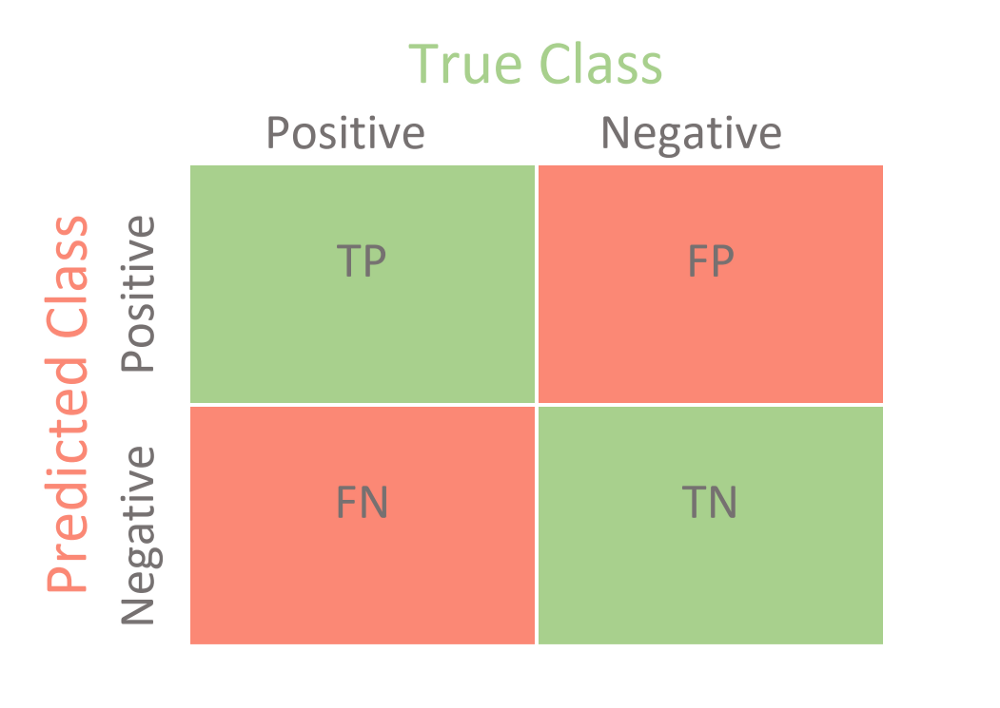
\includegraphics[scale=0.3]{pics/confusionmatrix.png}
			\captionof{figure}{$\csplit^{\pi}$}
		\end{center}
		\item ROC(Receiver Operating Characteristic): 
		\begin{enumerate}
			\item \textbf{Sensitivity} TPR (True Postive Rate): TP/(TP+FN), 代表分类器预测的正类中实际正实例占所有正实例的比例。
			\item \textbf{1-Specificity} FPR (False Postive Rate): FP/(FP+TN),代表分类器预测的正类中实际负实例占所有负实例的比例。
			\item \textbf{Specificity} TNR (True Negative Rate): TN/(FP+TN),代表分类器预测的负类中实际负实例占所有负实例的比例,TNR=1-FPR。
		\end{enumerate}
		\item AUC(Area Under the Curve): AUC用于衡量“二分类问题”机器学习算法性能(泛化能力).
		\item UAUC(Unbiased Area Under the Curve): 在每个用户维度做 AUC,在某一类用户主导的情况下,例如高热远多余低热用户的时候,UAUC 效果显然更好。
	\end{itemize}
	
\begin{center}
	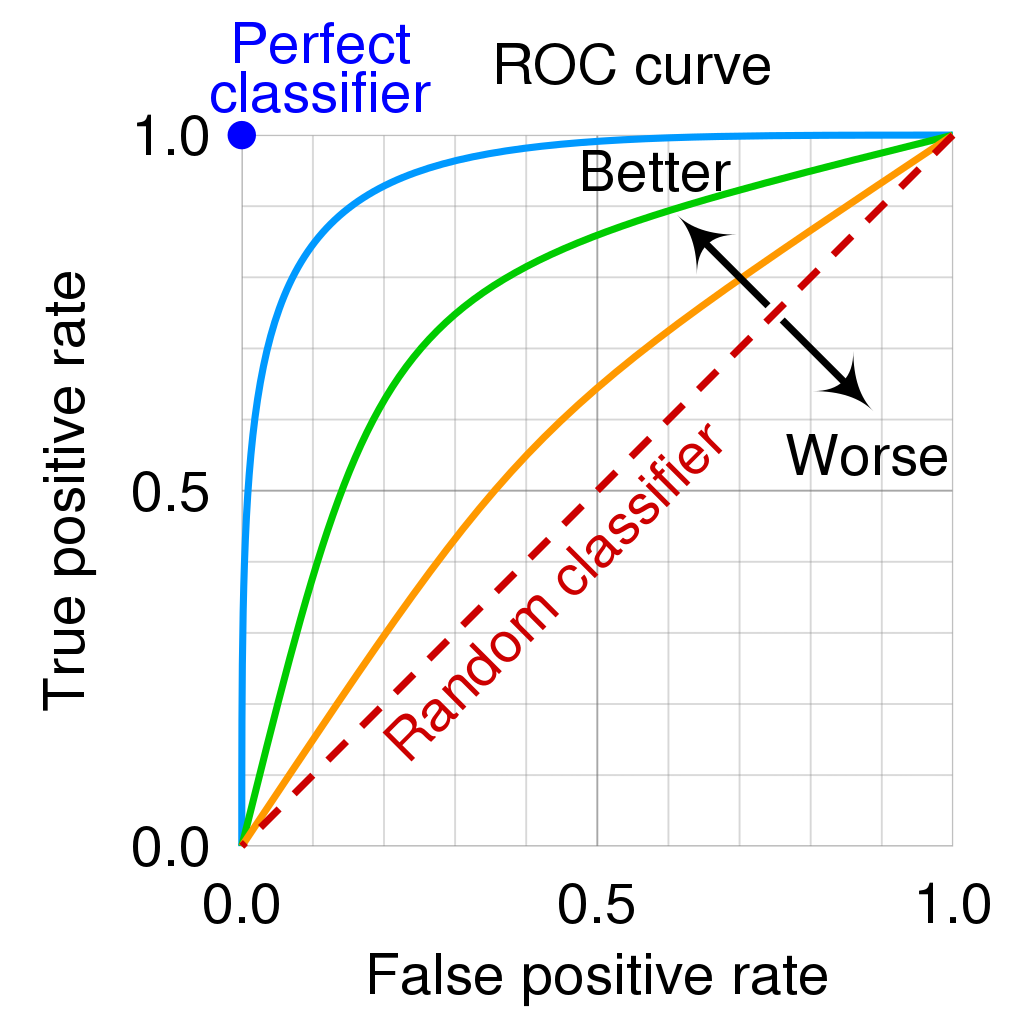
\includegraphics[scale=0.3]{pics/ROCAUC.png}
	\captionof{figure}{ROC  and AUC}
\end{center}

\begin{itemize}
	\item ROC 是就是 x 假阳率 vs y 真阳率
	\item Recall 和 Precision 是互相拮抗的,调整方法
	\begin{enumerate}
		\item 阈值:增大阈值,增加 Precision,减少 Recall;减小阈值,增加 Recall,减少 Precision
		\item 样本:如果新样本被正确预测为正类,精确率可能增加,召回率会增加;如果新样本被错误预测为负类(且假设不影响 FP),则精确率可能降低,召回率保持不变。
		\item 更改 loss function 的形式有可能有用
	\end{enumerate}
	\item Calibration: 以下是校准(calibration)与常见校准偏差解法的公式及描述:\textbf{校准的目的是将分类器的预测概率与实际标签的分布进行匹配。即使分类器经过良好的训练,其输出的概率(如 C)仍可能存在偏差。以 SVM 为例,SVM 的输出并不是预测的概率,因此,尽管预测分类可能准确,预测的平均值与真实正样本的占比之间仍会存在差距。因此,为了将预测值用作概率,需要进行校准。校准的逻辑类似于残差补全的思想,尽管在 ResNet 或 XGBoost 中,模型的提升是通过学习残差使损失逐渐减小,而校准的过程则是通过调整输出概率以提高其与真实标签的匹配度。换句话说,校准旨在将输出的概率分布拟合为真实值。常见的方法包括 Platt Scaling 和 Isotonic Regression,前者通过将 SVM 的对数几率拟合为一个逻辑函数,后者则通过逐段常数的方式调整输出概率,从而将 SVM 等模型的输出转换为可靠的概率预测。}
	
	\begin{enumerate}
		\item \textbf{校准公式}: \\
		校准曲线用于衡量分类器预测概率与实际观察到的结果的匹配度。如果模型被良好校准,预测事件发生的概率将与实际发生的概率一致。
		\begin{equation}
			C(f(x)) = P(Y=1 | \hat{p}=f(x))
		\end{equation}
		其中:
		\begin{itemize}
			\item \( C(f(x)) \) 是校准函数。
			\item \( f(x) \) 是预测的概率。
			\item \( P(Y=1 | \hat{p}=f(x)) \) 表示给定预测概率时事件发生的实际概率。
		\end{itemize}
		
		\item \textbf{校准偏差的常见解决方法}:
		\begin{enumerate}
			\item \textbf{Platt 缩放(Platt Scaling)}:
			\begin{equation}
				\hat{p} = \frac{1}{1 + \exp(Az + B)}
			\end{equation}
			其中:
			\begin{itemize}
				\item \( A \) 和 \( B \) 是通过训练数据学到的参数。
				\item \( z \) 是分类器的对数几率。
			\end{itemize}
			
			\item \textbf{等分回归(Isotonic Regression)}:
			\begin{equation}
				\hat{p}_{\text{calibrated}} = g(\hat{p})
			\end{equation}
			其中 \( g(\hat{p}) \) 是一个逐段常数、单调递增的函数,具体形式如下:
			\begin{equation}
				g(\hat{p}) = 
				\begin{cases}
					a_1, & \text{if } \hat{p} \in [p_0, p_1) \\
					a_2, & \text{if } \hat{p} \in [p_1, p_2) \\
					\vdots & \vdots \\
					a_n, & \text{if } \hat{p} \in [p_{n-1}, p_n]
				\end{cases}
			\end{equation}
			其中 \( p_0, p_1, \ldots, p_n \) 是分段点,\( a_1, a_2, \ldots, a_n \) 是对应的输出值。
			
			\item \textbf{Beta 校准(Beta Calibration)}:
			\begin{equation}
				\hat{p}_{\text{beta}} = \frac{1}{1 + \frac{1-\hat{p}}{\hat{p}} \cdot \exp(A + B \cdot \log(\hat{p}) + C \cdot \log(1-\hat{p}))}
			\end{equation}
			其中 \( A \)、\( B \) 和 \( C \) 是通过训练数据拟合的参数。
			\end{enumerate}
		\end{enumerate}
	
\end{itemize}

	
	\begin{table*}[h]\centering
		\caption{Regression 分类模型评估}
		\label{Regression Evaluation}
		\ra{1.1}
		\begin{tabular}{@{}ccc@{}}
			\toprule
			指标&  描述 & Scikit-learn函数 \\
			\midrule
			Mean Square Error (MSE, RMSE) &  平均方差 & from $sklearn.metrics$ import $mean\_squared\_error$\\
			Absolute Error (MAE, RAE) &  绝对误差 & from $sklearn.metrics$ import $mean\_absolute\_error$ or $median\_absolute\_error$\\
			R-Squared &  R平方值 & from $sklearn.metrics$ import $r2\_score$\\
			\bottomrule
		\end{tabular}
	\end{table*}

\section{统计基础知识}

\subsection{Bootstrap}
自助法, 拔靴法 Bootstrap Method,Bootstrapping或自助抽样法, 均匀的有放回抽样(sample size $n$, 做$n$次有放回的抽样,得到新的数据集),根本原因在于如果总体是正态分布的
(\href{}{百度自助法}),那么sample distribution 也是正态分布的。根据 $(1-\frac{1}{n})^n\to \frac{1}{e}\approx 0.368$, 那么大概会有1/3 的样本不会出现在训练集里。

\begin{itemize}
	\item 跟cross validation 一样,是模型检验的一种方式
	\item 优点: 每次1/3 当成 test set
	\item 缺点: 这样产生的训练集的数据分布和原数据集的不一样了, 只是在当数据集非常大,且高斯分布的时候会近似,会引入估计偏差。
	\item 用途:自助法在数据集较小,难以有效划分训练集/验证集时很有用;此外,自助法能从初始数据集中产生多个不同的训练集,这对集成学习(bagging(bootstrap aggregating的缩写,也称作“套袋法”))等方法有很大的好处。
	\item 总结:Bootstraping通过重复抽样,避免了Cross Validation造成的样本减少的问题。其次,Bootstraping也可以用于随机创造数据。比如,随机森林算法就是从原始训练数据中,用bootstrap sampling的方法有放回地随机抽取k个新的自助样本集,并由此构建k棵分类回归树。但由于其训练集有重复数据,这会改变数据的分布,因而导致训练结果有估计偏差,因此这种方法不是很常用,除非数据量真的很少。
	\item \href{https://www.cnblogs.com/HuZihu/p/11145518.html}{boosting 博客}, \href{https://www.cnblogs.com/HuZihu/p/9368362.html}{Cross Validation 博客}
\end{itemize}

\section{特征工程}

\begin{itemize}
	\item 编码方式 \href{https://blog.csdn.net/m0_61796189/article/details/127332472}{【机器学习】特征工程中常见的特征编码}
	\begin{enumerate}
		\item One-hot encoder: 特征多的时候维度大(可以尝试用 PCA 降维度),维度固定时有冲突,而且不可学习; 但是对于不可比较的类别特征,比如 country 就还行
		\item Label encoder: 变成 0,1,2, etc., 没有标签的具体含义,适用于支持类比性算法的模型,XGboot
		\item Ordinal encoder: 拍个顺,本科0,研究生1,博士2 等等,依赖先验知识
		\item Frequence encoder: 出现几次就用几,对于离群值敏感,而且容易出现冲突
	 	\item  Mean encoder: target 频次的 mean, 也容易出现冲突
	 	\item 分箱取整缩放
	\end{enumerate}
\end{itemize}

\section{Generative VS discriminative}

\begin{itemize}
	\item Generative: learn $\P(x,y)$, i.e. GDA, Native bayes. 学习联合分布
	\item Discriminative: learn $\P(y|x)$, Regression, SVMs. 学习边界
	\item \href{https://www.zhihu.com/question/20446337}{Generative VS discriminative}
	\item \href{https://stats.stackexchange.com/questions/91484/do-discriminative-models-overfit-more-than-generative-models}{why generative mode 更不容 overfit}
	\item Discriminative: 直接学习 $p(y|x)$, 学习 decision boundary, i.e. Regression, SVM
	\item Generative: 学习 $p(x|y)$ 然后用bayesian 推出 $p(y|x)$, 学习的其实是 data 的分布,i.e. GDA, Naive Bayes
\end{itemize}

\subsection{Generative 1. Gaussian Discriminant Analysis}

label 0 和 1 服从 $Ber(P)$, 在固定的 label 下所有 data 服从 Gaussian(不同的mean), 对于所有 parameter的 MLE 都是 canonical unbiased estimator。

\subsection{Generative 2. Naive Bayes }
\begin{itemize}
\item Assumption: The Naive Bayes model supposes that the features of each data point are all independent。\href{https://zhuanlan.zhihu.com/p/37575364}{为什么一定要是独立的}
\item MLE 就是 highest count。
\item Naive Bayes is widely used for text classification and spam detection.
\end{itemize}











\section{Generalization}

模型泛化的能力决定了模型能多有用。
$$Error = Bia + Variance$$

\begin{center}
	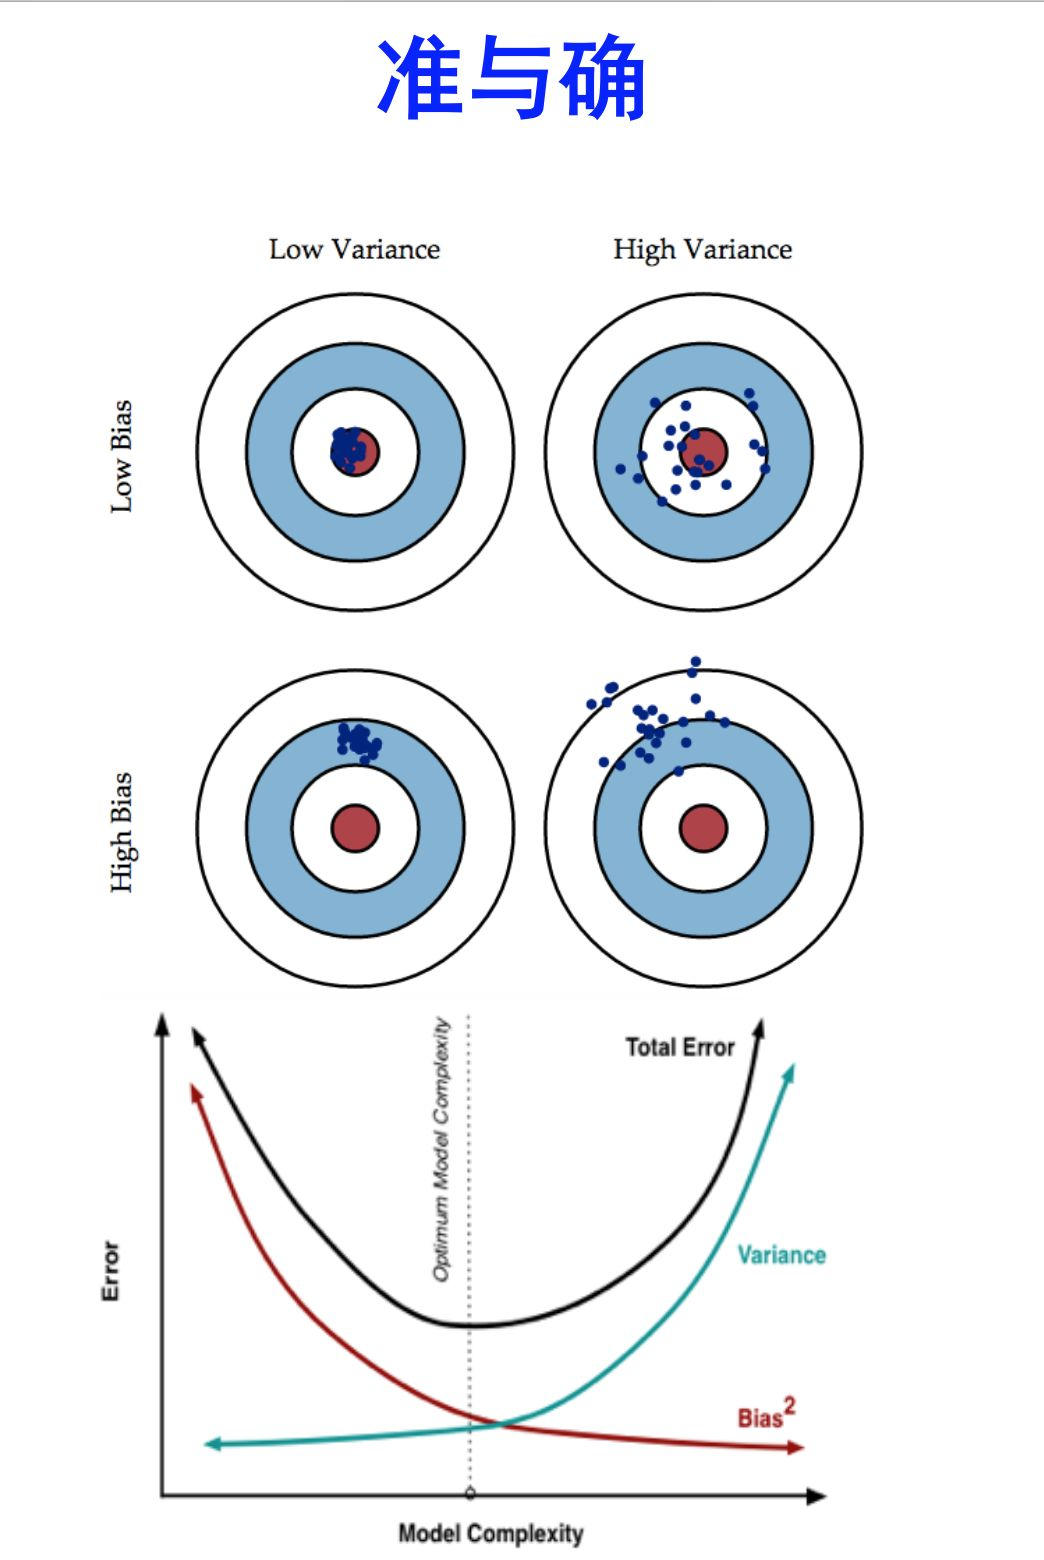
\includegraphics[scale=0.35]{pics/bias_var.jpg}
	\captionof{figure}{Bias n Variance}
\end{center}

\begin{itemize}
	\item Variance 过大, 是模型 overfitting 
	\item 利用 k-fold  cross validation 一定会增加bias,因为利用所有数据训练一定是 bias最低的, 不过相应的 variance 会降低。 Trade off is art.
	\item \href{http://scott.fortmann-roe.com/docs/BiasVariance.html}{Bias and Variance trade-off}
\end{itemize}
	
	
	\section{Regularization}
	\begin{itemize}
		\item 最主要的目的: 解决 overfitting
		\item 同时满足了 Occam's Razor
		\item \textbf{l1 (Lasso)}:  稀疏化,特征的自动选取,模型解释性
		\item \textbf{l2 (Ridge)}: 不会稀疏, 但是robust 很好,同时对于 outlier 更敏感
		\item 对于 logistic regression, 特殊的解释就是,l1,l2 其实是 prior distribution,l1对应的是 Lapacian l2 对应的是 Gaussian
	\end{itemize}



	\section{linear Regression}
	
	\begin{itemize}
		\item 5个基本假设: 线性可加性,线性独立,误差 $\epsilon$ 的相互独立, 误差的方差为常数,而且误差出现正态分布
		\item \href{https://blog.csdn.net/Noob_daniel/article/details/76087829}{如何利用残差等检验模型是否是线性的}
	\end{itemize}


	\section{聚类}
	\subsection{Kmeans}
	\begin{itemize}
		\item \href{https://www.jianshu.com/p/8f19b04fc0eb?utm_campaign=maleskine&utm_content=note&utm_medium=seo_notes&utm_source=recommendation}{Kmeans特点}, 更加泛化的
		\href{https://zhuanlan.zhihu.com/p/78311644}{EM特点}
	\end{itemize}

	\section{Logistic Regression}
	
	\href{https://zhuanlan.zhihu.com/p/74874291}{Logistic Regression 详解} 
	Classification, supervised, discriminative, Linear regression 是 maximal entropy 在 二分的特例, loss 是 -log likelihood, 其实就是 logistic loss(cross entropy)。参数模型。
	\begin{itemize}
		\item 逻辑回归模型中的最大化似然函数与最小化损失函数的等价性: 逻辑回归用于二分类问题,其输出为样本属于某一类的概率。假设我们有一个样本特征 $ x $ 和其对应的标签 $ y \in \{0, 1\} $,逻辑回归模型的形式为:
		
		\begin{equation}
			P(y=1|x) = \sigma(w^T x) = \frac{1}{1 + e^{-w^T x}}
		\end{equation}
		
		这里,$ w $ 是模型的权重,$ \sigma $ 是逻辑函数。
		\item 最大化似然函数: 似然函数定义为在给定参数 $ w $ 的情况下,观测到的样本数据的概率。对于 $ n $ 个样本,其似然函数可以表示为:
		
		\begin{equation}
			L(w) = \prod_{i=1}^{n} P(y_i|x_i) = \prod_{i=1}^{n} \sigma(w^T x_i)^{y_i} (1 - \sigma(w^T x_i))^{1 - y_i}
		\end{equation}
		
		为了方便计算,我们通常取对数,得到对数似然函数:
		
		\begin{equation}
			\ell(w) = \log(L(w)) = \sum_{i=1}^{n} \left( y_i \log(\sigma(w^T x_i)) + (1 - y_i) \log(1 - \sigma(w^T x_i)) \right)
		\end{equation}
		\item 最小化损失函: 逻辑回归中的损失函数通常定义为负对数似然损失(Cross-Entropy Loss):
		
		\begin{equation}
			J(w) = -\frac{1}{n} \sum_{i=1}^{n} \left( y_i \log(\sigma(w^T x_i)) + (1 - y_i) \log(1 - \sigma(w^T x_i)) \right)
		\end{equation}
		\item 等价关系的解释: 
		- **最大化似然与最小化损失**:从对数似然函数中可以看出,最大化似然函数相当于最小化负对数似然损失。因此,在训练逻辑回归模型时,最大化似然函数和最小化损失函数是等价的。
		
		- **优化目标**:在优化过程中,最大化 $ \ell(w) $(对数似然)等同于最小化 $ J(w) $(损失函数),因此在使用梯度下降等优化算法时,选择其中一种方法都能得到相同的参数估计。
		
		- **结论**:综上所述,\textbf{逻辑回归模型中,最大化似然函数和最小化损失函数实际上是两个不同的优化目标,但它们在数学上是等价的}。这使得在实现逻辑回归模型时,可以灵活选择优化方法。
	\end{itemize}
		
		
		
		
	
	
	\subsection{与 SVM 对比}
	\begin{itemize}
		\item \textbf{相同}:
		\begin{enumerate}
			\item 都是分类算法,本质上都是在找最佳分类超平面;
			\item 都是监督学习算法;
			\item 都是判别式模型,判别模型不关心数据是怎么生成的,它只关心数据之间的差别,然后用差别来简单对给定的一个数据进行分类;
			\item 都可以增加不同的正则项。
		\end{enumerate}
		\item \textbf{不同}:
		\begin{enumerate}
			\item LR 是一个统计的方法,SVM 是一个几何的方法;
			\item SVM 的处理方法是只考虑 Support Vectors,也就是和分类最相关的少数点去学习分类器。而逻辑回归通过非线性映射减小了离分类平面较远的点的权重,相对提升了与分类最相关的数据点的权重;
			\item 损失函数不同:LR 的损失函数是交叉熵,SVM 的损失函数是 HingeLoss,这两个损失函数的目的都是增加对分类影响较大的数据点的权重,减少与分类关系较小的数据点的权重。对 HingeLoss 来说,其零区域对应的正是非支持向量的普通样本,从而所有的普通样本都不参与最终超平面的决定,这是支持向量机最大的优势所在,对训练样本数目的依赖大减少,而且提高了训练效率;
			\item LR 是参数模型,SVM 是非参数模型,参数模型的前提是假设数据服从某一分布,该分布由一些参数确定(比如正太分布由均值和方差确定),在此基础上构建的模型称为参数模型;非参数模型对于总体的分布不做任何假设,只是知道总体是一个随机变量,其分布是存在的(分布中也可能存在参数),但是无法知道其分布的形式,更不知道分布的相关参数,只有在给定一些样本的条件下,能够依据非参数统计的方法进行推断。所以 LR 受数据分布影响,尤其是样本不均衡时影响很大,需要先做平衡,而 SVM 不直接依赖于分布;
			\item LR 可以产生概率,SVM 不能;
			\item LR 不依赖样本之间的距离,SVM 是基于距离的;
			\item LR 相对来说模型更简单好理解,特别是大规模线性分类时并行计算比较方便。而 SVM 的理解和优化相对来说复杂一些,SVM 转化为对偶问题后,分类只需要计算与少数几个支持向量的距离,这个在进行复杂核函数计算时优势很明显,能够大大简化模型和计算。
		\end{enumerate}
	\end{itemize}
	
	\section{SVM}
	\href{https://zhuanlan.zhihu.com/p/49331510}{SVM 详解} 
	把所有点分成 $x_i^\intercal W+b\ge 1$ 和 $x_i^\intercal  W+b\le -1$ 两部分,并要求两平行直线距离最短
	\begin{equation}
		L(W,b,\alpha) = \frac{1}{2} \lVert W \rVert^2 - \sum\limits_{i=1}^n \alpha_i [y_i(x_i^\intercal W+b)-1]
	\end{equation}

解为
\begin{equation}
\begin{cases}
	\hat{W} = \sum\limits_{i\in SV} \hat{\alpha_i} y_i x_i\\
	\hat{b} = y_j - \sum\limits_{i\in SV} \hat{\alpha_i} y_i x_i^\intercal x_i\\
	f(x) = sign (\sum\limits_{i\in SV} \hat{\alpha_i}y_ix^\intercal x_i +\hat{b})
	\end{cases}
\end{equation}
只与 support vector 有关。需要的点比较少。决策函数为
\begin{itemize}
	\item 线性时 
	\begin{equation}
		f(x) = \hat{W}^\intercal x + b
	\end{equation}
	\item 非线性 kernel 时
	\begin{equation}
		f(x) = \sum_{i=1}^{n} \alpha_i y_i K(x_i, x) + b
	\end{equation}
\end{itemize}



\subsection{Soft Margin}
对于软性间隔问题(soft margin): 
\begin{equation}
	\underset{W,b}{\min} \frac{1}{2}\lVert W \rVert^2 +C\sum\limits_{i=1}^n \max\big(0,1-y_i(x_iW+b)\big)
\end{equation}

前一项可以理解为“结构风险(structural risk)”,用来描述所求模型的某些性质(SVM就是要求间隔最大);第二项称为“经验风险(empirical risk)”
	
\subsection{Nonlinear}

Kernel trick. 决策函数可以变为
i.e. 用 $[K(x,z)]$ 去代替 $x^\intercal x$
\begin{itemize}
	\item 多项式核:$K(x,z) = (x\cdot z + 1)^p$
	\item 高斯核(RBF: Radial Basis Function, 除了前面的常数项,类Gaussian Kernel):$K(x,z) = \exp(-\frac{\lVert x-z \rVert}{2\sigma^2})$
\end{itemize}

\subsection{SVM 的 SGD 的实现}
\begin{itemize}
	\item \href{http://liuhongjiang.github.io/tech/blog/2013/01/31/svm-pegasos/}{Pegasos算法} \item\href{https://blog.csdn.net/qq_53123067/article/details/136060974}{机器学习 | 一文看懂SVM算法从原理到实现全解析}
	\item \href{https://blog.csdn.net/sinat_27612639/article/details/70037499}{svm随机次梯度下降算法-pegasos}
	\item \href{https://www.deep-ml.com/problem/Pegasos%20Kernel%20SVM%20Implementation}{ml-deep pegasos}
\end{itemize}

\subsection{总结}
\begin{itemize}
	\item 优点:
	\begin{enumerate}
		\item 由于SVM是一个凸优化问题,所以求得的解一定是全局最优而不是局部最优。
		\item 不仅适用于线性线性问题还适用于非线性问题(用核技巧)。
		\item 拥有高维样本空间的数据也能用SVM,这是因为数据集的复杂度只取决于支持向量而不是数据集的维度,这在某种意义上避免了“维数灾难”。
		\item 理论基础比较完善(例如神经网络就更像一个黑盒子)。
	\end{enumerate}
	\item 缺点:
	\begin{enumerate}
		\item 二次规划问题求解将涉及m阶矩阵的计算(m为样本的个数), 因此SVM不适用于超大数据集。(SMO算法可以缓解这个问题)
		\item 只适用于二分类问题。(SVM的推广SVR也适用于回归问题;可以通过多个SVM的组合来解决多分类问题)。
	\end{enumerate}
\end{itemize}


\section{分类问题和回归问题的却别}
\begin{itemize}
	\item 分类问题 的 loss 应该是 cross entropy, 这取决于本身分类问题的返回应该是不同类别的概率,那么天生应该比较的是概率分布是否相似。如果用 MSE + softmax 会出现梯度消失的情况
\end{itemize}

\section{优化器的选择}
\subsection{GD 家族}
\begin{table}[h]
	\centering
	\caption{GD、SGD 和 Mini-batch SGD 的优缺点}
	\begin{tabular}{@{}p{2.5cm} p{5cm} p{5cm}@{}}
		\toprule
		方法                  & 优点                                                     & 缺点                                                        \\ \midrule
		\textbf{GD}              & - 全局精确更新\newline - 稳定的收敛                          & - 计算代价高\newline - 内存占用大\newline - 收敛速度慢                \\ \midrule
		\textbf{SGD}             & - 更新速度快\newline - 内存占用小\newline - 更容易跳出局部最优解   & - 更新噪声大\newline - 收敛精度差\newline - 较小的学习率,并且可能采用学习率衰减            \\ \midrule
		\textbf{Mini-batch SGD}   & - 计算效率较高\newline - 收敛过程较平稳\newline - 利用硬件并行   & - 仍有一定噪声\newline - 批次大小调整困难                      \\ \bottomrule
	\end{tabular}
\end{table}
\subsection{SGD 到 Adam}

\href{https://zhuanlan.zhihu.com/p/32626442}{SGD-ADAM} 
\href{https://zhuanlan.zhihu.com/p/32488889}{SGD, ADAM 主要区别} : 加入了一阶和二阶动量,一阶解决了陷入local min 和震荡的问题, 二阶动量继承了历史上的gradient 改动,自适应,改动越多的我们不希望改动太多。同时二阶动量和是一个窗口,避免了出现学习率为0的情况。

\begin{enumerate}
	\item 核心思路:动量法和 RMSProp 
	\item 动量法: 一阶动量平滑了梯度的方向
	\item RMSProp: 二阶动量避免了大步长更新带来的不稳定性
	\item beta 的滑动窗口平均,使得近期 grad 的影响更大
\end{enumerate}



\section{Tree-based and ensemble methods}

\subsection{Decision Tree}

决策树的构造就是进行属性选择度量确定各个特征属性之间的拓扑结构, 决策树的属性分裂选择是”贪心“算法,也就是没有回溯的。选择每次让信息熵增加最多的 feature 作为 parent node,同时也可以搜索分裂点
\begin{itemize}
	\item 优点
	\begin{itemize}
		\item 可解释性强
		\item 可以同时处理数值和类别特征
	\end{itemize}
	\item 缺点
	\begin{itemize}
		\item 过度拟合:噪音数据, 缺少代表性数据, 多重比较
		\item 大量的 if else,不好并行
		\item 不稳定
	\end{itemize}
\end{itemize}
\begin{itemize}
	\item 设定阈值及终止条件
	\item 可以用 K-Fold Cross Validation
	\item 划分点的方法:\href{https://blog.csdn.net/zhihua_oba/article/details/72230427}{回归树和决策树划分节点的方法}
	\item 树模型可以一定程度上对于不平衡数据不敏感,本质上不平衡数据的问题在于没办法对于小类别有很好的估计。但是树模型可以通过类似信息增益比等划分节点的方式一定程度上注重小类别。
	\item \href{https://zhuanlan.zhihu.com/p/341598480}{DT 总结}
	\begin{enumerate}
		\item IC3: 用信息熵的增益
		\item IC4.5: 避免某些feature 下面分类过多,做归一化,信息熵的增益比
		\item CART: 分类问题采用基尼系数来选择最优特征和分裂点,回归问题采用平方误差的总值(总方差)来选择最优特征和分裂点
	\end{enumerate}
	\item 解决过拟合的方法, regularization: pruning \href{https://towardsdatascience.com/3-techniques-to-avoid-overfitting-of-decision-trees-1e7d3d985a09}{DT overfitting}
	\begin{enumerate}
		\item pre-pruning: early stop, max depth, max num of samples
		\item post-pruning: grow to full, then 同时平衡num of node 和 误差 \href{https://www.cnblogs.com/shayue/p/jue-ce-shu-fang-zhi-guo-ni-he.html}{前后剪纸示意图}
	\end{enumerate}
\end{itemize}

\subsection{Random Forest(Bagging)}
步骤
\begin{enumerate}
	\item 一个样本容量为N的样本,有放回的抽取N次,每次抽取1个,最终形成了N个样本。这选择好了的N个样本用来训练一个决策树,作为决策树根节点处的样本。
	\item 当每个样本有M个属性时,在决策树的每个节点需要分裂时,随机从这M个属性中选取出m个属性,满足条件 $m<<M$。然后从这m个属性中采用某种策略(比如说信息增益)来选择1个属性作为该节点的分裂属性。
	\item 决策树形成过程中每个节点都要按照步骤2来分裂(很容易理解,如果下一次该节点选出来的那一个属性是刚刚其父节点分裂时用过的属性,则该节点已经达到了叶子节点,无须继续分裂了)。一直到不能够再分裂为止。注意整个决策树形成过程中没有进行剪枝。
	\item 按照步骤1~3建立大量的决策树,这样就构成了随机森林了。
\end{enumerate}
优点
\begin{enumerate}
	\item 它可以出来很高维度(特征很多)的数据,并且不用降维,无需做特征选择
	\item 它可以判断特征的重要程度
	\item 可以判断出不同特征之间的相互影响
	\item 不容易过拟合
	\item 训练速度比较快,容易做成并行方法
	\item 实现起来比较简单
	\item 对于不平衡的数据集来说,它可以平衡误差。
	\item 如果有很大一部分的特征遗失,仍可以维持准确度。
\end{enumerate}

缺点
\begin{enumerate}
	\item 随机森林已经被证明在某些噪音较大的分类或回归问题上会过拟合。
	\item 对于有不同取值的属性的数据,取值划分较多的属性会对随机森林产生更大的影响,所以随机森林在这种数据上产出的属性权值是不可信的
\end{enumerate}

\subsection{Boosting}
步骤
\begin{enumerate}
	\item 先通过对N个训练数据的学习得到第一个弱分类器h1;
	\item 将h1分错的数据和其他的新数据一起构成一个新的有N个训练数据的样本,通过对这个样本的学习得到第二个弱分类器h2;
	\item 将h1和h2都分错了的数据加上其他的新数据构成另一个新的有N个训练数据的样本,通过对这个样本的学习得到第三个弱分类器h3;
	\item 最终经过提升的强分类器$h_final$=Majority Vote(h1,h2,h3)。即某个数据被分为哪一类要通过h1,h2,h3的多数表决。
	\item \href{https://blog.csdn.net/brucewong0516/article/details/78656299}{bagging 和 boosting 的优缺点}, 典型案例 \href{https://zhuanlan.zhihu.com/p/130461268}{GBDT}, 和他的进阶版本 \href{https://www.zhihu.com/question/41354392}{xgboost}
\end{enumerate}



\subsection{Adaboost}
High weights are put on errors to improve at the next boosting step.

\section{PCA and ICA}
\subsection{PCA}
\begin{enumerate}
	\item 对所有的样本 $D_{n\times m} = (x_1,\cdots,x_m) $ 进行中心化
	\item 计算样本的协方差矩阵 $(XX^\intercal)_{n\times n}$
	\item 对矩阵  $XX^\intercal_{n\times n}$ 进行特征值分解
	\item 取出最大的$n' < n$个特征值对应的特征向量 $w_1,\cdots,w_{n'}$, 将所有的特征向量标准化后,组成特征向量矩阵$W_{nn'}$。
	\item 对样本集中的每一个样本 ,转化为新的样本 $(z_i)_{n'\times 1} = W^\intercal x_i$
	\item 得到输出样本集 $D' = (z_i,\cdots,z_m)_{n'\times m}$
	\item PCA 对于稀疏特征有作用,避免了由于数据缺失导致特征系数而影响了模型效果
\end{enumerate}

\subsection{ICA: Independent component analysis}
步骤 \href{https://www.cnblogs.com/jerrylead/archive/2011/04/19/2021071.html}{ICA} 
一般只对Gaussian denoise 比较有效。


\section{Unsupervised}
Motivation: The goal of unsupervised learning is to find hidden patterns in unlabeled data.

\subsection{Expectation-Maximization: EM}
步骤 \href{https://zhuanlan.zhihu.com/p/78311644}{EM} 

\begin{itemize}
	\item Expectation: 对于初始的 $\theta$, 算出数据对应的 posterior distribution
	\item 对于所有cluster ,按权重用 MLE 更新 $\theta$
\end{itemize}

\subsection{K-means}
选定K 个簇,选取中中心,每一个点选择最近的中心,划分完更新中心,知道终止条件打成。

\begin{itemize}
	\item 需要用户事先指定类簇个数K
	\item 聚类结果对初始类簇中心的选取较为敏感;
	\item 容易陷入局部最优; 
	\item 只能发现球型类簇;
\end{itemize}

\subsection{Hierarchical Clustering 层聚类}

跟 NJ method 思路一致,适用于树状结构。
\begin{itemize}
	\item Single Linkage: 两个组合数据点中距离最近的两个数据点间的距离作为这两个组合数据点的距离。 两个不同组数据点可能由于其中的某个极端的数据点距离较近而组合在一起。
	\item Complete Linkage: 将两个组合数据点中距离最远的两个数据点间的距离作为这两个组合数据点的距离。 两个相似组数据点可能由于其中的某个极端的数据点距离较远而分开。
	\item 平均值,计算量大,但是少偏差。
\end{itemize}

\section{Entropy}
\href{https://www.iitg.ac.in/cseweb/osint/slides/Anasua_Entropy.pdf}{Entropy} 
\begin{equation}
	H(P,Q) = H(P) + KL(P||Q)
\end{equation}

	
\subsection{定义}
	
	\begin{enumerate}
		\item \textbf{熵 (Entropy)}: 对于离散随机变量 \( X \) 的熵定义为:
		\begin{equation}
			H(X) = -\sum_{i} p(x_i) \log p(x_i)
		\end{equation}
		其中 \( p(x_i) \) 是随机变量 \( X \) 的概率分布。
		
		\item \textbf{交叉熵 (Cross Entropy)}: 随机变量 \( X \) 和 \( Y \) 的交叉熵定义为:
		\begin{equation}
			H(p, q) = -\sum_{i} p(x_i) \log q(x_i)
		\end{equation}
		其中 \( p(x_i) \) 是真实分布,\( q(x_i) \) 是模型分布。
		
		\item \textbf{KL 散度 (KL Divergence  aka Relative Entropy)}: 随机变量 \( X \) 和 \( Y \) 之间的 KL 散度定义为:
		\begin{equation}
			D_{KL}(p \parallel q) = \sum_{i} p(x_i) \log \frac{p(x_i)}{q(x_i)} = H(p, q) - H(p)
		\end{equation}
	\end{enumerate}
	
	\subsection{Cross Entropy 和 Relative Entropy 的对比}
	
	 为什么 Logistic Regression 使用交叉熵而不是 KL 散度
	 
	 \begin{enumerate}
	 	\item KL 散度用于衡量两个完整概率分布之间的差异,而分类问题中的真实标签并不构成概率分布。
	 	\item 交叉熵在分类问题中更直接、更有效地计算模型输出概率与真实标签之间的误差.
	 	\item 使用交叉熵损失简化了优化过程,与 Logistic 回归的输出形式(Sigmoid 概率)高度匹配。
	 \end{enumerate}
	 
	
	
	
	\begin{table}[h]
		\centering
		\caption{Relative Entropy(相对熵) vs Cross Entropy(交叉熵)总结}
		\begin{tabular}{@{}p{3cm} p{6cm} p{6cm}@{}}
			\toprule
			指标 & KL散度(相对熵) & 交叉熵 \\ \midrule
			\textbf{定义} 
			& 衡量两个分布之间的差异,用于描述模型估计与真实分布的偏差 
			& 衡量模型分布与真实分布之间的总损失,包含模型误差和数据本身的不确定性 \\ \midrule
			\textbf{公式} 
			& $D_{KL}(P \parallel Q) = \sum P(x) \log \frac{P(x)}{Q(x)}$ 
			& $H(P, Q) = -\sum P(x) \log Q(x)$ \\ \midrule
			\textbf{是否包含 $H(P)$} 
			& 不包含 
			& 包含 $H(P)$ 和 $D_{KL}(P \parallel Q)$ \\ \midrule
			\textbf{应用场景} 
			& 用于优化模型概率输出,使其更接近真实分布 
			& 在分类问题等监督学习中作为常用的损失函数 \\ \midrule
			\textbf{直观理解} 
			& 度量模型估计的分布与真实分布之间的差异 
			& 衡量模型预测误差与数据固有不确定性的综合损失 \\ \bottomrule
		\end{tabular}
	\end{table}
	
	
	
	\subsection{KL 的正定性}
	
	为了证明 KL 散度 \( D_{KL}(p \parallel q) \geq 0 \),我们可以使用 Jensen 不等式。以下是证明过程:
	
	1. \textbf{定义}: 由于 \( q(x_i) > 0 \),我们可以考虑:
	\begin{equation}
		D_{KL}(p \parallel q) = \sum_{i} p(x_i) \log \frac{p(x_i)}{q(x_i)} = \sum_{i} p(x_i) \left( \log p(x_i) - \log q(x_i) \right)
	\end{equation}
	
	2. \textbf{应用 Jensen 不等式}:
	设 \( f(x) = \log x \),这是一个凹函数,因此根据 Jensen 不等式:
	\begin{equation}
		f\left( \sum_{i} p(x_i) q(x_i) \right) \geq \sum_{i} p(x_i) f(q(x_i))
	\end{equation}
	于是我们得到:
	\begin{equation}
		\log \left( \sum_{i} p(x_i) q(x_i) \right) \geq \sum_{i} p(x_i) \log q(x_i)
	\end{equation}
	
	3. \textbf{利用上面的不等式}:
	这表明:
	\begin{equation}
		D_{KL}(p \parallel q) \geq 0
	\end{equation}
	
	综上所述,我们可以得出结论:
	\begin{equation}
		D_{KL}(p \parallel q) \geq 0
	\end{equation} 
	
	并且等号成立当且仅当 \( p = q \) 时。
	



\section{NN}
\subsection{Activation function}
\begin{itemize}
	\item ReLu over Sigmoid:
	\begin{itemize}
		\item Sigmoid:梯度消失,求导缓慢,0点非对称导致梯度下降不均衡
		\item ReLU: 稀疏大部分 Neuron 不激活,求导快,正部梯度一直为1,0点虽然不可导但是可以利用单边的导数; 负值如果没有梯度可以用 leaky ReLU 加一个很小的梯度
	\end{itemize}
	\item 常见激活函数的导数
	\begin{itemize}
		\item \textbf{Sigmoid 激活函数}
		\begin{equation}
			\sigma(x) = \frac{1}{1 + e^{-x}}
		\end{equation}
		\begin{equation}
			\sigma'(x) = \sigma(x)(1 - \sigma(x))
		\end{equation}
		
		\item \textbf{Tanh 激活函数}
		\begin{equation}
			\tanh(x) = \frac{e^{x} - e^{-x}}{e^{x} + e^{-x}} = \frac{2}{1 + e^{-2x}} - 1
		\end{equation}
		\begin{equation}
			\tanh'(x) = 1 - \tanh^2(x)
		\end{equation}
		
		\item \textbf{ReLU 激活函数}
		\begin{equation}
			\text{ReLU}(x) = \max(0, x)
		\end{equation}
		\begin{equation}
			\text{ReLU}'(x) = 
			\begin{cases} 
				1 & \text{if } x > 0 \\ 
				0 & \text{if } x \leq 0 
			\end{cases}
		\end{equation}
		
		\item \textbf{Leaky ReLU 激活函数}
		\begin{equation}
			\text{Leaky ReLU}(x) = 
			\begin{cases} 
				x & \text{if } x > 0 \\ 
				\alpha x & \text{if } x \leq 0 
			\end{cases}
		\end{equation}
		其中 $\alpha$ 是一个很小的常数(通常设置为 0.01)。
		\begin{equation}
			\text{Leaky ReLU}'(x) = 
			\begin{cases} 
				1 & \text{if } x > 0 \\ 
				\alpha & \text{if } x \leq 0 
			\end{cases}
		\end{equation}
		
		\item \textbf{Softmax 激活函数}
		\begin{equation}
			\text{softmax}(z_i) = \frac{e^{z_i}}{\sum_{j} e^{z_j}}
		\end{equation}
		\begin{equation}
			\text{softmax}'(z_i) = \text{softmax}(z_i)(1 - \text{softmax}(z_i)) \quad \text{for } i = j
		\end{equation}
		\begin{equation}
			\text{softmax}'(z_i) = -\text{softmax}(z_i)\text{softmax}(z_j) \quad \text{for } i \neq j
		\end{equation}
	\end{itemize}
\end{itemize}

\subsection{初始化}
\begin{itemize}
	\item 部分参数例如 bias 初始置0的话可能使得网络收敛比较慢
	\item 如果全部置 0 的话,模型就是对称的,那么本质上就相当于只有一个神经元了!
\end{itemize}

\subsection{Dropout layer}

\href{https://zhuanlan.zhihu.com/p/38200980}{Dropout} 
为了解决 overfitting 的问题,从 bagging 的角度来说,自网络的ensemble。


\subsection{NLP}
\begin{itemize}
	\item 基础知识 \href{https://zhuanlan.zhihu.com/p/61635013}{word2vec} , 最基本的利用skip gram, CBOW, 一个是当前词预测周围,一个是周围词汇预测当前
	\href{https://zhuanlan.zhihu.com/p/32829048}{N gram}
	\item \href{https://blog.csdn.net/hfutdog/article/details/96479716}{RNN and LSTM}, RNN 只有短期记忆,LSTM有长期
	\item seq2seq 利用encoder 和 decoder, 但是同样面临遗忘的问题
	\item attention 机制解决了 seq2seq 的遗忘问题,代价是巨大的计算量,因为每一次解码都与要计算与之前所有 encoder 状态向量的相似度 \href{https://www.youtube.com/watch?v=XhWdv7ghmQQ&t=0s}{注意力机制视频}
	\item \href{https://blog.csdn.net/None_Pan/article/details/106485896}{Transformer 相比 RNN 和 LSTM 的优势}, 更无序,句子整体处理
	\item \href{https://www.zhihu.com/question/439243827}{关于 Transformer 的总结}
\end{itemize}

\section{NLP 类别}
\begin{itemize}
	\item N-gram:  markov 假设,通过统计前后出现pair的频率计算一句话的概率。\textbf{用于句子生成,文本补全,机器翻译}
	\item BOW:  Bag of words, 统计句子里面的词频生成 vector,太稀疏太大还没有前后语意关系
	\item TF-IDF(Term Frequency-Inverse Document Frequency): 是一种常见的文本表示方法,广泛用于\textbf{信息检索}和\textbf{文本挖掘},特别是文本的特征提取和相似性计算任务。它通过衡量一个词在文档中的重要性来表示词与文本的关联程度。
		
		\begin{itemize}
			\item \textbf{TF(Term Frequency)}:词频,表示某个词在文档中出现的次数。
			\item \textbf{IDF(Inverse Document Frequency)}:逆文档频率,表示某个词在整个文档集合中出现的频率。IDF 通过降低那些在大多数文档中都频繁出现的词(如“the”、“is”等)的权重,突出那些更能区分文档的词。
		\end{itemize}
		
		对于某个词 $t$ 在文档 $d$ 中的 TF-IDF 计算公式为:
		
		\[
		\text{TF-IDF}(t, d) = \text{TF}(t, d) \times \text{IDF}(t)
		\]
		
		其中:
		\begin{itemize}
			\item \textbf{TF}:词 $t$ 在文档 $d$ 中出现的频率。
			\item \textbf{IDF}:定义为 
			\[
			\text{IDF}(t) = \log \left( \frac{N}{1 + n_t} \right)
			\]
			其中 $N$ 是文档总数,$n_t$ 是包含词 $t$ 的文档数。
		\end{itemize}
	\item BM25: TF-IDF 升级版,直接计算 query 和文档分数,综合了文档长度
	\item Bert and Transformer: 可以进行文本分类,语句生成,匹配等更多功能; attention 的 QKV 线性捕捉全局依赖,和 MLP 的特征交叉结合,生成更好的 embedding, 然后比较 CLS 的相似性 cos。
	
\end{itemize}


\section{数学问题, 概率论}

\begin{enumerate}
	\item 20 个人生日不相同的概率是多少?如何估计:准确答案 $1-\frac{365!}{365^n (365-20)!}$, 近似的话,首先设 $Y_{i,j}$ 表示 i,j 生日相同,所有的 $Y_{i,j}$ are almost independent, then $Y_{i,j}\sim Ber(1/365)$, sum of bernulli $\to Binomial(n^2/2, 1/365)$, and Bin 的极限是 $Possion(\lambda)$,  
	\begin{equation}
		\lambda = \E[Pos] \approx \E[Bin] = \frac{n^2}{2}\frac{1}{365}=n^2/730
	\end{equation}
	Then 
	\begin{equation}
		\P[\sum Y_{i,j} = 0] = \exp^{-\lambda} = \exp^{-\frac{n^2}{730}}
	\end{equation}
\href{https://www.zhihu.com/question/372854533}{生日问题,小数定律}
\end{enumerate}


\section{推荐系统}
\begin{itemize}
	\item 链路:召回 $\to$ 粗排 $\to$ 精排 $\to$ 重排
	\begin{itemize}
		\item \href{https://blog.csdn.net/qq_27590277/article/details/120681803}{链路讲解}
	\end{itemize}

	\item 常见的 embedding 手段:w2v, item2v, graph embedding(i.e.\href{https://zhuanlan.zhihu.com/p/64200072}{w2v to DeepWalk to Node2v to EGES(适合冷启动)})
	
	\item \textbf{召回模型} 从NFEP的视角理解召回。
	
	Near——定义向量距离近,取决于不同的召回方式。
	
	Far——定义向量距离远,取决于负样本的采样方式。
	
	Embedding——如何生成embedding,这被归结到用户/物品画像的问题。
	
	Pairwise-loss——召回阶段无法追求预测值与标签值的绝对准确性,所以往往采用Pairwise(user,item+,item-)追求排序之间的相对准确性。 \href{https://www.zhihu.com/question/315120636/answer/1687203383}{召回策略}
	\begin{enumerate}
		\item 以矩阵分解为基础的:\href{https://lumingdong.cn/recommendation-algorithm-based-on-matrix-decomposition.html}{矩阵分解详解,实际业务中已经过时}
		\item 因子分解机(FM): \href{https://www.cnblogs.com/techflow/p/14893349.html}{FM 的基本原理}, 如何将交叉项计算复杂度降到$O(kn)$,以及如何解决了 LR 里面面临的1: 特征不够,如需要人工制作特征; 2: 稀疏特征的问题。 \href{https://zhuanlan.zhihu.com/p/58160982}{FM 为什么会解决多回路召回的问题}
		\item 双塔 DSSM \href{https://zhuanlan.zhihu.com/p/430503952}{双塔介绍}, \href{https://www.6aiq.com/article/1589485687711}{双塔在实际业务中的应用}
		\begin{itemize}
			\item 后期融合模型,Pros: 适合召回,快速, Cons: 没有用户特征和物品特征的交互
			\item 正负样本选取,pointwise, pairwise and listwise 三种训练 \href{https://zhuanlan.zhihu.com/p/111636490}{三种训练的优劣}
			\item 简单负样本:未被召回的,困难负样本:未进入粗排, 非常困难负样本:未进入精排
			\item 曝光但未点击的样本,只可以作为排序模型的负样本,但不可以作为retrival 的负样本,原因很简单,没被点击的原因只是因为兴趣没有那么高,但不代表没有兴趣!!
			\item DSSM 实现的时候,用户向量是随时计算的,而物品向量是pre cal的,既平衡了计算难度,同时也符合人是动态变化的,但是物品是相对稳定的
		\end{itemize}
	\end{enumerate}
	
	\item \textbf{推荐模型}:
	\begin{enumerate}
		\item LS-PLM(MLR大规模分段线性模型): 阿里曾用,先聚类,再在聚类的基础上对每一类做 LR。 Pros: 快 Cons: 对非线性拟合有限
	\end{enumerate}
	
	\item \textbf{深度网络}: \href{https://cloud.tencent.com/developer/article/1824345}{线性模型,深度模型,树模型,attention 模型1},和 \href{https://cloud.tencent.com/developer/article/1824350?from=article.detail.1824345}{线性模型,深度模型,树模型,attention 模型2}。总结贴 \href{https://zhuanlan.zhihu.com/p/409610336}{深度学习网络总结},包括传统的\href{https://www.youtube.com/watch?v=kY4W46MQqsg&list=PLvOO0btloRntAi-VnV06M1Bu0X1xljUUP&index=13}{多目标模型}和 \href{https://www.youtube.com/watch?v=JIEwaPARjfk&list=PLvOO0btloRntAi-VnV06M1Bu0X1xljUUP&index=14}{MMoE}
	\begin{enumerate}
		\item embedding: LR 到 FM/FFM/biFFM 充分利用了交叉特征
		\item DNN 下的: FNN PNN 和 DeepCrossing 的通用Pros: 抓住了高阶交叉特征,cons: 对于低阶特征利用不足。 简单来说,\textbf{线性模型以浅层形式直接学习稀疏组合特征权重,对训练数据中出现过的组合特征具有很好的记忆能力。而深度模型,稀疏特征被映射成低维稠密embedding向量,随后在深层全连接网络中获得充分交互,对具体的特征组合的“记忆”能力会减弱,但换来了更好的泛化效果}。
		\begin{itemize}
			\item FNN(Factorisation-machine supported Neural Networks,以 FM 的隐藏层作为输入)
			\item PNN(Product-based Neural Network, 在 FNN 的基础上增加了 product layer)
			\item DeepCrossing (借助了 ResNet residual unit 的概念,将传统的 MLP 改为了 residual unit)
		\end{itemize}
		\item Wide$\&$Deep: 联合学习,LR(Wide 记忆性) + DNN(Deep, 泛化能力)。Wide 和 Deep 输入值是不同的,因为 LR 需要人工构造特征。衍生品
		\begin{itemize}
			\item DeepFM: FM + DNN
			\item DeepCross Network(DCN): Cross(多项式快速计算,O(d)) + DNN。 $x_{i+1} = x_0x_i^\intercal W_i  + x_i$
			\item Neural Factorization Machines(NFM): DNN 会梯度/爆炸和过拟合等问题 。NFM的主要改进点是,引入Bi-Interaction Pooling层,替代经典DNN的concat层,在底层增加足够的特征交互信息后,再馈入到MLP网络做进一步的高阶非线性建模。
		\end{itemize}
	\item Attention 机制:
	\begin{itemize}
		\item AFM: 相比于 NFM, 通过 attention net 计算 attention 权重因子。cons: 缺少高阶交叉信息
	\end{itemize}
	\item 精排 LHUC(PPNet Parameter Personalized Net): 从语音识别的 LHUC 出发,将个性化(UserID) 的embedding 用来放大或者缩小物品(IternID)的 embedding,从而实现个性化
	\item FiBiNET: SeNet本质上同过压缩再放缩实现对 feature fieldwise 的加权 $+$ Bilinear cross。具体结构为 concatenation + bilinear cross + SeNet bilinear cross
	\item 序列模型(Last N):
	\begin{itemize}
		\item 简单的 last N 取平均作为feature,平均池化,作为用户特征,可以放入召回,粗排,精排
		\item DIN: 利用 attention 机制,计算候选物品与 last N 的相似度然后做加权平均。 因为要用到候选物品只适用于精排
		\item SIM: 在DIN 模型的基础上,试图增加 n,并且减少last n 中与候选物品完全不相关的物品,减少计算成本, last N to top K. Hard search 和 soft search 用来找 top K, soft 结果更好,但是计算成本更大。同时加入物品交互时间信息。
	\end{itemize}
	\end{enumerate}

	\item 推荐链路中的重排:多样性抽样,尽量多利用内容特征(CV, NLP)而不是用ID 从 双塔中学习的特征,因为头部现象明显,对于长尾和新进物品都不好。
	\begin{enumerate}
		\item MMR: Maximal Marginal Relevance : 通过 $\lambda$ 控制一遍满足和 query 的相关性,一遍降低同推荐列表里最相似物品的相关性, 实践中可以通过滑动窗口增加相似性的有效性(如果对于所有物品,那么相似性很容易是1)。 同时可以加入规则约束同时优化。
		\item DPP: Determinental Point Process local repulsive 的性质, 使得 sampling 的时候不会过于相似。 快手加Hulu: \href{https://proceedings.neurips.cc/paper/2018/file/dbbf603ff0e99629dda5d75b6f75f966-Paper.pdf}{DPP}: 用 $\log(\det V^\intercal V)$ 代替了MMR 中的相似惩罚项(常规的DPP), 创新在于提出了贪心思路下快速的行列式计算
		\item \href{https://www.zhihu.com/question/62962281}{MMR, DPP 总结 1} 和 \href{https://zhuanlan.zhihu.com/p/411553235}{MMR, DPP 总结 2}
	\end{enumerate}
	
	\item 冷启动的问题:
	\begin{enumerate}
		\item 评价指标:对于 UGC(user generated content) 的平台, 区别于 PGC(platform generated content) , 可以通过作者侧指标(渗透率),用户侧指标(新物品消费指标,大盘指标 DAU etc), 还有内容指标(高热笔记占比)
		\item 召回通道:ItemCF 不行,因为没有用户交互,直接用双塔也不好,因为用户item embedding 不对 
		\begin{itemize}
			\item 改进双塔,Item embedding 从其他相似物品中学习
			\item 通过类目和关键词
			\item 聚类召回,把所有item cluster 然后召回每个感兴趣 cluster 中最新的几个
			\item Look alike 人群扩散
		\end{itemize}
	\end{enumerate}
	
	\item 业界实例:
	\begin{enumerate}
		\item Facebook: \href{https://arxiv.org/pdf/2006.11632.pdf}{FB 2020}
		\item Youtube: \href{https://storage.googleapis.com/pub-tools-public-publication-data/pdf/6c8a86c981a62b0126a11896b7f6ae0dae4c3566.pdf}{YouTube 2019}
		\item 快手: 
		\begin{itemize}
			\item \href{https://www.51cto.com/article/644214.html}{快手的 PPNet}, 源自 \href{https://www.youtube.com/watch?v=TxIedW94hu0&list=PLvOO0btloRntAi-VnV06M1Bu0X1xljUUP&index=20}{Learning Hidden Unit Contribution(LHUC)}
			\item 快手加Hulu: \href{https://proceedings.neurips.cc/paper/2018/file/dbbf603ff0e99629dda5d75b6f75f966-Paper.pdf}{DPP}
		\end{itemize}
		
		
		
		\item 微博 \href{https://arxiv.org/pdf/1905.09433.pdf}{FiBiNET}
		\item 阿里 \href{https://arxiv.org/pdf/1706.06978.pdf}{DIN}, \href{https://arxiv.org/pdf/2006.05639.pdf}{SIM}, \href{https://github.com/wzhe06/Reco-papers/blob/master/Embedding/[Alibaba%20Embedding]%20Billion-scale%20Commodity%20Embedding%20for%20E-commerce%20Recommendation%20in%20Alibaba%20(Alibaba%202018).pdf}{EGES}
	\end{enumerate}
\end{itemize}

\section{搜索系统}
\subsection{文本查询分类}

文本查询可以分为头部查询、中间查询和尾部查询。每种情况下通常使用的不同方法如下:

\begin{enumerate}
	\item \textbf{头部查询(Head Queries)}:
	\begin{itemize}
		\item \textbf{特征选择和加权}:对于高频查询,通常会使用特征选择技术来识别关键字,并为其分配较高的权重。
		\item \textbf{搜索引擎优化(SEO)}:应用广泛的SEO策略,以确保这些查询在搜索结果中优先展示。
		\item \textbf{聚合和推荐}:利用历史数据和用户行为进行结果聚合和个性化推荐。
	\end{itemize}
	
	\item \textbf{中间查询(Torso Queries)}:
	\begin{itemize}
		\item \textbf{语义理解}:使用自然语言处理(NLP)技术来理解查询的意图,并提供相关结果。
		\item \textbf{上下文建模}:根据用户的上下文信息(如位置、搜索历史)调整查询结果。
		\item \textbf{混合搜索策略}:结合关键词匹配和语义匹配,提供更相关的搜索结果。
	\end{itemize}
	
	\item \textbf{尾部查询(Tail Queries)}:
	\begin{itemize}
		\item \textbf{长尾优化}:对于这些低频查询,采用特定的内容推荐策略,以确保即使是冷门查询也能找到相关结果。
		\item \textbf{用户反馈机制}:通过用户的点击率和反馈数据,逐步优化尾部查询的结果。
		\item \textbf{内容扩展}:通过增加相关内容或使用用户生成的内容来增强搜索引擎的结果,以满足更广泛的查询。
	\end{itemize}
\end{enumerate}

	

\section{训练架构}
\begin{itemize}
	\item\href{https://www.bilibili.com/video/BV1pR4y1h7TR/?spm_id_from=333.337.search-card.all.click&vd_source=7a090a6e6fbf50b4a73122127ec9b13b}{Jax}	: Google 可以用 cpu 和 gpu 加速 
\end{itemize}

\section{链接}
\begin{itemize}
	\item \href{https://www.1point3acres.com/bbs/thread-713903-1-1.html}{Amazon 八股文1},and  \href{https://northern-dracopelta-98c.notion.site/5b22e124e16d4b2d937940367ca20eb0?v=19feabb85e9e4b54bc498579b3c7f1c5&p=e74be76a2d3c4746b94e54d190100e4e&pm=s}{八股文1 noion}
	\item \href{https://www.1point3acres.com/bbs/thread-714090-1-1.html}{八股文2}
	\item \href{https://www.1point3acres.com/bbs/thread-927931-1-1.html}{最新 Pinterest OA 面经}
	\item \href{https://www.1point3acres.com/bbs/thread-714558-1-1.html}{八股文3}
	\item\href{https://zhuanlan.zhihu.com/p/422464069}{推荐系统面试集锦}
\end{itemize}





	 \end{CJK}  
\end{document}